% ====================================================================================
\appendixchapter{工程专题}{工程专题}
% ====================================================================================

\noindent\textit{本附录收录各章的工程类延伸内容}：它们原是第 13、6、8、9 章的扩展阅读，篇幅长、偏实践，放在正文里会把主线撑得很不均匀。各节相互独立，需要时再翻。前三节配合第 13 章的有限元：\textbf{大规模线性方程组的求解艺术}讲直接法、共轭梯度、预条件、多重网格与条件数；\textbf{CPU 并行计算的真正含义}讲并行到底并行了什么、为什么加核不一定加速；\textbf{流固耦合有限元}完整复现 Turek--Hron FSI2 基准算例。后三节分别配合第 6、8、9 章：\textbf{从旋转矩阵到三维重建}从 $SO(3)$ 与指数映射讲到从图像重建三维结构；\textbf{Python 表达式求值}解释解释器怎样把 \texttt{x*x+2*x+1} 变成一棵计算图；\textbf{用 SB3 训练经典控制任务}介绍 Stable Baselines3 的安装、训练与调参。

% ====================================================================================
\section*{大规模线性方程组的求解艺术}
\addcontentsline{toc}{section}{大规模线性方程组的求解艺术}
% ====================================================================================

\begin{tcolorbox}[colback=gray!5, colframe=gray!50, title=本节导读]
有限元方法的最后一步是求解线性方程组 $KU = F$。这看起来很简单——不就是解个方程吗？

但当工程师模拟一架波音787的应力时，这个方程组可能有\textbf{上亿个未知数}。如何高效求解？答案涉及到一些深刻的数学概念：条件数、稀疏性、并行计算和预条件子。

更令人惊讶的是，这些概念在现代机器学习中同样重要——神经网络的训练本质上也是在求解大规模方程组！
\end{tcolorbox}

% ------------------------------------------------------------------------------------
\subsection*{一、条件数：方程组的“健康指标”}

\subsubsection*{一个令人困惑的现象}

考虑两个看起来很相似的方程组：

\noindent\begin{minipage}[t]{0.48\textwidth}
\textbf{方程组 A}
\[
\begin{pmatrix} 1 & 0 \\ 0 & 1 \end{pmatrix}
\begin{pmatrix} x \\ y \end{pmatrix}
= \begin{pmatrix} 1 \\ 1 \end{pmatrix}
\]
解：$x = 1, y = 1$

如果右边有小扰动 $(1.01, 0.99)$：

解变成 $x = 1.01, y = 0.99$

\textbf{扰动 1\%，解也变化 1\%}
\end{minipage}
\hfill
\begin{minipage}[t]{0.48\textwidth}
\textbf{方程组 B}
\[
\begin{pmatrix} 1 & 1 \\ 1 & 1.0001 \end{pmatrix}
\begin{pmatrix} x \\ y \end{pmatrix}
= \begin{pmatrix} 2 \\ 2.0001 \end{pmatrix}
\]
解：$x = 1, y = 1$

如果右边有小扰动 $(2.01, 2.0001)$：

解变成 $x = 101, y = -99$

\textbf{扰动 0.5\%，解变化 10000\%！}
\end{minipage}

\vspace{0.5cm}

为什么方程组 B 如此“敏感”？这就是\textbf{条件数}要回答的问题。

\subsubsection*{条件数的定义}

\begin{keyformula}[title=条件数]
矩阵 $A$ 的\textbf{条件数}定义为最大奇异值与最小奇异值之比：
\begin{equation}
\kappa(A) = \|A\| \cdot \|A^{-1}\| = \frac{\sigma_{\max}(A)}{\sigma_{\min}(A)}
\end{equation}

对于对称正定矩阵（如有限元刚度矩阵），它就是最大特征值与最小特征值之比：
\begin{equation}
\kappa(K) = \frac{\lambda_{\max}(K)}{\lambda_{\min}(K)}
\end{equation}
\end{keyformula}

条件数衡量的是方程组把输入扰动放大了多少倍：$\kappa \approx 1$ 时方程组“健康”，对扰动不敏感；$\kappa \gg 1$ 时方程组“病态”，小扰动可能导致大误差；到了 $\kappa = \infty$，矩阵奇异，方程没有唯一解。

\begin{figure}[htbp]
\centering
\begin{tikzpicture}[scale=1.5]
    % 左边：良态矩阵
    \begin{scope}
        \node[font=\bfseries] at (1, 2.3) {良态 $\kappa \approx 1$};
        \draw[->] (0, 0) -- (2.2, 0) node[right] {$x$};
        \draw[->] (0, 0) -- (0, 2.2) node[above] {$y$};
        
        % 单位圆
        \draw[blue, thick] (1, 1) circle (0.7);
        \node[blue] at (1, 0.1) {输入扰动};
        
        % 输出也是圆（差不多大小）
        \draw[red, thick, dashed] (1, 1) ellipse (0.8 and 0.6);
        \node[red] at (1.8, 1.8) {输出误差};
    \end{scope}
    
    % 右边：病态矩阵
    \begin{scope}[xshift=4cm]
        \node[font=\bfseries] at (1, 2.3) {病态 $\kappa \gg 1$};
        \draw[->] (0, 0) -- (2.2, 0) node[right] {$x$};
        \draw[->] (0, 0) -- (0, 2.2) node[above] {$y$};
        
        % 单位圆
        \draw[blue, thick] (1, 1) circle (0.3);
        \node[blue] at (1, 0.5) {输入扰动};
        
        % 输出是扁长椭圆
        \draw[red, thick, dashed, rotate around={30:(1,1)}] (1, 1) ellipse (1.5 and 0.15);
        \node[red] at (2.2, 1.8) {输出误差};
        \node[red, font=\scriptsize] at (2.2, 1.5) {被放大！};
    \end{scope}
\end{tikzpicture}
\caption{条件数的几何意义：病态矩阵把圆形扰动拉成细长椭圆}
\end{figure}

\subsubsection*{有限元刚度矩阵的条件数}

有限元刚度矩阵的条件数与网格步长 $h$ 密切相关：

\begin{keytheorem}[title=刚度矩阵条件数估计]
对于一维 Poisson 方程的有限元刚度矩阵：
\begin{equation}
\kappa(K) \sim O\left(\frac{1}{h^2}\right)
\end{equation}

网格加密一倍（$h \to h/2$），条件数增大约 4 倍！
\end{keytheorem}

\textbf{为什么会这样？}

回顾刚度矩阵的三对角结构：
\[
K = \frac{1}{h}
\begin{pmatrix}
2 & -1 & & \\
-1 & 2 & -1 & \\
& \ddots & \ddots & \ddots \\
& & -1 & 2
\end{pmatrix}
\]

这个矩阵的特征值可以精确计算：
\begin{equation}
\lambda_k = \frac{4}{h} \sin^2\left(\frac{k\pi h}{2}\right), \quad k = 1, 2, \ldots, N-1
\end{equation}

当 $k = 1$ 时正弦的自变量很小，$\sin^2 x \approx x^2$，于是最小特征值 $\lambda_1 \approx \frac{4}{h} \cdot \frac{\pi^2 h^2}{4} = \pi^2 h$；当 $k = N-1$ 时自变量接近 $\pi/2$，最大特征值 $\lambda_{N-1} \approx \frac{4}{h}$。两者相除：
\[
\kappa(K) = \frac{\lambda_{\max}}{\lambda_{\min}} \approx \frac{4/h}{\pi^2 h} = \frac{4}{\pi^2 h^2} \sim O(h^{-2})
\]

\begin{physicalmeaning}
条件数有直接的物理含义。刚度矩阵的\textbf{最大特征值}对应高频振动模式——相邻节点反向运动，局部而快速；\textbf{最小特征值}对应低频振动模式——整体缓慢变形，全局而慢速。网格越细，高频和低频的差距越大，条件数也就越大。这就像一根弦：基频（整体振动）和高次谐波（局部振动）的频率差距可以很大。
\end{physicalmeaning}

\subsubsection*{条件数对计算的影响}

条件数影响两件事。第一是直接求解的精度：用高斯消元法求解时，舍入误差会被放大约 $\kappa$ 倍，如果 $\kappa = 10^{10}$，双精度浮点数（约 15 位有效数字）就只能保证约 5 位精度。第二是迭代求解的速度：很多迭代算法（如共轭梯度法）的收敛速度与条件数直接相关，所需的迭代次数是 $O(\sqrt{\kappa})$ 量级，$\kappa = 10^6$ 就意味着需要约 $1000$ 次迭代。

% ------------------------------------------------------------------------------------
\subsection*{二、稀疏矩阵：大自然的礼物}

\subsubsection*{什么是稀疏矩阵？}

\begin{definition}[稀疏矩阵]
如果一个 $n \times n$ 矩阵中非零元素的个数远小于 $n^2$（通常是 $O(n)$ 量级），我们称它为\textbf{稀疏矩阵}。
\end{definition}

有限元刚度矩阵就是典型的稀疏矩阵！

\begin{example}[波音787的有限元模型]
有限元与飞机结构的缘分由来已久（第 13 章开头提到的 1956 年波音机翼分析），我们也用一架飞机来估算规模。假设模型有 $n = 10^7$（一千万）个节点。若把刚度矩阵当作稠密矩阵存储，就有 $10^7 \times 10^7 = 10^{14}$ 个元素，占 $10^{14} \times 8$ 字节 $= 800$ TB，根本存不下；求解的运算量 $O(n^3) = 10^{21}$ 次，也根本算不完。但它其实是稀疏的：三维问题里每行只有约 30 个非零元，总共 $3 \times 10^8$ 个非零元，只需约 $2.4$ GB 内存；配上稀疏求解器，求解就变得可行。
\end{example}

\subsubsection*{三对角矩阵：最简单的稀疏结构}

一维有限元产生的三对角矩阵是最简单的稀疏矩阵：

\[
K = \begin{pmatrix}
a_1 & c_1 & & & \\
b_2 & a_2 & c_2 & & \\
& b_3 & a_3 & c_3 & \\
& & \ddots & \ddots & \ddots \\
& & & b_n & a_n
\end{pmatrix}
\]

\textbf{Thomas 算法}（追赶法）可以在 $O(n)$ 时间内求解！

\noindent\textbf{算法：Thomas 算法（三对角系统求解）}

\begin{enumerate}
  \item \textbf{前向消元（从上到下）}：对 $i=2,\dots,n$，令 $w = b_i / a_{i-1}$，然后更新 $a_i \leftarrow a_i - w \cdot c_{i-1}$ 与 $f_i \leftarrow f_i - w \cdot f_{i-1}$。这一步以第 $i-1$ 行为基准，消掉第 $i$ 行的 $b_i$，右端项做同样的线性组合。
  \item \textbf{回代（从下到上）}：先算 $x_n = f_n / a_n$——链条最末端最简单，从这里开始把信息传回去；再对 $i = n-1, n-2, \dots, 1$ 依次算 $x_i = (f_i - c_i \cdot x_{i+1}) / a_i$。
\end{enumerate}

\begin{insightbox}
\textbf{Thomas 算法的本质}：

三对角系统就像一条链：
\[
\bullet - \bullet - \bullet - \bullet - \bullet
\]

每个节点只与相邻节点耦合。

前向消元将链条“一节节剪断”，回代将解“一节节传回”。

本质上就是一种线性结构的动态规划。
\end{insightbox}


\subsubsection*{带状矩阵与块三对角矩阵}

二维和三维问题的刚度矩阵虽然不是三对角，但仍有规律的稀疏结构：

\begin{figure}[htbp]
\centering
\begin{tikzpicture}[scale=0.52]

    % -------------------------------
    % 一维：三对角
    % -------------------------------
    \begin{scope}[xshift=0cm]
        \node[font=\bfseries] at (2.5, 6) {一维：三对角};
        \draw[gray] (0,0) rectangle (5,5);

        % 主对角
        \foreach \i in {0,...,4} {
            \fill[blue!60] (\i, 4-\i) rectangle ++(1,1);
        }
        % 上下对角
        \foreach \i in {0,...,3} {
            \fill[blue!30] (\i+1, 4-\i) rectangle ++(1,1);
            \fill[blue!30] (\i, 3-\i) rectangle ++(1,1);
        }

        \node at (2.5, -0.8) {\small 带宽 = 1};
    \end{scope}


    % -------------------------------
    % 二维：带状
    % -------------------------------
    \begin{scope}[xshift=8.5cm]
        \node[font=\bfseries] at (3, 6) {二维：带状};
        \draw[gray] (0,0) rectangle (6,6);

        % 主对角
        \foreach \i in {0,...,5} {
            \fill[blue!60] (\i, 5-\i) rectangle ++(1,1);
        }
        % 近对角
        \foreach \i in {0,...,4} {
            \fill[blue!30] (\i+1, 5-\i) rectangle ++(1,1);
            \fill[blue!30] (\i, 4-\i) rectangle ++(1,1);
        }
        % 远对角（来自另一方向）
        \foreach \i in {0,...,2} {
            \fill[blue!15] (\i+3, 5-\i) rectangle ++(1,1);
            \fill[blue!15] (\i, 2-\i) rectangle ++(1,1);
        }

        \node at (3, -0.8) {\small 带宽 $\approx \sqrt{n}$};
    \end{scope}


    % -------------------------------
    % 三维：更宽的带
    % -------------------------------
    \begin{scope}[xshift=17cm]
        \node[font=\bfseries] at (3.5, 6) {三维：更宽的带};
        \draw[gray] (0,0) rectangle (7,7);

        % 主对角
        \foreach \i in {0,...,6} {
            \fill[blue!60] (\i, 6-\i) rectangle ++(1,1);
        }

        % 逐步扩散的带状
        \foreach \d in {1,2,3} {
            \pgfmathsetmacro{\alpha}{60-15*\d}
            \foreach \i in {0,...,\numexpr6-\d} {
                \fill[blue!\alpha] (\i+\d, 6-\i) rectangle ++(1,1);
                \fill[blue!\alpha] (\i, 6-\i-\d) rectangle ++(1,1);
            }
        }

        \node at (3.5, -0.8) {\small 带宽 $\approx n^{2/3}$};
    \end{scope}

\end{tikzpicture}
\caption{不同维度问题的刚度矩阵稀疏结构}
\end{figure}


\textbf{带宽}决定了直接求解所需的计算量：

\begin{center}
\begin{tabular}{c|c|c|c}
\toprule
问题维度 & 带宽 $b$ & 求解复杂度 & $n = 10^6$ 时 \\
\midrule
一维 & $O(1)$ & $O(n)$ & $10^6$ 次运算 \\
二维 & $O(\sqrt{n})$ & $O(n \cdot b^2) = O(n^2)$ & $10^{12}$ 次运算 \\
三维 & $O(n^{2/3})$ & $O(n \cdot b^2) = O(n^{7/3})$ & $10^{14}$ 次运算 \\
\bottomrule
\end{tabular}
\end{center}

这就是为什么\textbf{大规模三维问题必须用迭代法}。

% ------------------------------------------------------------------------------------
\subsection*{三、并行计算：分而治之}

\subsubsection*{为什么三对角求解难以并行？}

Thomas 算法虽然快（$O(n)$），但它是\textbf{串行}的：前向消元的第 $i$ 步依赖第 $i-1$ 步的结果，回代的第 $i$ 步又依赖第 $i+1$ 步的结果。就像多米诺骨牌，必须一个接一个倒下，不能跳跃。

\begin{figure}[htbp]
\centering
\begin{tikzpicture}[scale=0.8]
    % 串行
    \node[font=\bfseries] at (3, 2) {串行 Thomas 算法};
    \foreach \i in {1,...,6} {
        \draw[thick, fill=blue!30] (\i, 0) rectangle ++(0.6, 1);
        \node at (\i+0.3, 0.5) {\small $\i$};
    }
    \draw[->, thick, red] (1.3, 0.5) -- (1.7, 0.5);
    \draw[->, thick, red] (2.3, 0.5) -- (2.7, 0.5);
    \draw[->, thick, red] (3.3, 0.5) -- (3.7, 0.5);
    \draw[->, thick, red] (4.3, 0.5) -- (4.7, 0.5);
    \draw[->, thick, red] (5.3, 0.5) -- (5.7, 0.5);
    \node at (3.5, -0.8) {\small 必须按顺序执行};
\end{tikzpicture}
\end{figure}

\subsubsection*{域分解：把问题切开}

一个聪明的想法：把计算域\textbf{分成几块}，每块独立求解，然后把边界“缝合”起来。

\begin{figure}[htbp]
\centering
\begin{tikzpicture}[scale=1.2]
    % 原始问题
    \begin{scope}
        \node[font=\bfseries] at (2, 1.5) {原始问题};
        \draw[thick] (0, 0) -- (4, 0);
        \foreach \i in {0,...,8} {
            \fill (\i*0.5, 0) circle (2pt);
        }
        \node at (2, -0.5) {8个节点，一个方程组};
    \end{scope}
    
    % 箭头
    \draw[->, very thick] (4.5, 0) -- (5.5, 0);
    
    % 分解后
    \begin{scope}[xshift=6cm]
        \node[font=\bfseries] at (2, 1.5) {域分解};
        
        % 子域1
        \draw[thick, blue] (0, 0) -- (1.8, 0);
        \foreach \i in {0,...,3} {
            \fill[blue] (\i*0.5, 0) circle (2pt);
        }
        \node[blue] at (0.9, 0.4) {子域1};
        
        % 子域2
        \draw[thick, red] (2.2, 0) -- (4, 0);
        \foreach \i in {5,...,8} {
            \fill[red] (\i*0.5, 0) circle (2pt);
        }
        \node[red] at (3.1, 0.4) {子域2};
        
        % 界面
        \draw[thick, green!60!black, dashed] (1.8, -0.3) -- (2.2, -0.3);
        \fill[green!60!black] (2, 0) circle (3pt);
        \node[green!60!black] at (2, -0.7) {界面};
        
        \node at (2, -1.2) {两个小方程组 + 界面条件};
    \end{scope}
\end{tikzpicture}
\caption{域分解的基本思想}
\end{figure}

\subsubsection*{Schur 补：界面上的方程}

设原方程组为：
\[
\begin{pmatrix}
A_{11} & A_{12} & 0 \\
A_{21} & A_{22} & A_{23} \\
0 & A_{32} & A_{33}
\end{pmatrix}
\begin{pmatrix}
u_1 \\ u_\Gamma \\ u_2
\end{pmatrix}
=
\begin{pmatrix}
f_1 \\ f_\Gamma \\ f_2
\end{pmatrix}
\]

其中 $u_1, u_2$ 是两个子域的内部节点，$u_\Gamma$ 是界面节点。我们的目标是把内部节点消掉，得到一个只含界面未知量 $u_\Gamma$ 的小方程组。

\paragraph{推导 Schur 补}

把矩阵方程展开成三个方程：
\begin{align}
A_{11} u_1 + A_{12} u_\Gamma &= f_1 \tag{子域1内部} \\
A_{21} u_1 + A_{22} u_\Gamma + A_{23} u_2 &= f_\Gamma \tag{界面} \\
A_{32} u_\Gamma + A_{33} u_2 &= f_2 \tag{子域2内部}
\end{align}

\textbf{第一步}：从方程(1)解出 $u_1$（把 $u_\Gamma$ 当作已知量）
\[
u_1 = A_{11}^{-1}(f_1 - A_{12} u_\Gamma)
\]

\textbf{第二步}：从方程(3)解出 $u_2$（把 $u_\Gamma$ 当作已知量）
\[
u_2 = A_{33}^{-1}(f_2 - A_{32} u_\Gamma)
\]

\textbf{第三步}：把 $u_1, u_2$ 代入方程(2)，消去内部自由度
\begin{align*}
A_{21} \cdot \underbrace{A_{11}^{-1}(f_1 - A_{12} u_\Gamma)}_{u_1} + A_{22} u_\Gamma + A_{23} \cdot \underbrace{A_{33}^{-1}(f_2 - A_{32} u_\Gamma)}_{u_2} &= f_\Gamma
\end{align*}

展开并整理（把 $u_\Gamma$ 的项放到左边，常数项放到右边）：
\begin{equation}
\underbrace{\left(A_{22} - A_{21}A_{11}^{-1}A_{12} - A_{23}A_{33}^{-1}A_{32}\right)}_{S} u_\Gamma = \underbrace{f_\Gamma - A_{21}A_{11}^{-1}f_1 - A_{23}A_{33}^{-1}f_2}_{\tilde{f}_\Gamma}
\end{equation}
左边的矩阵 $S$ 叫作 \textbf{Schur 补}，右边的 $\tilde{f}_\Gamma$ 是修正后的右端项。这就是我们要的界面方程 $S u_\Gamma = \tilde{f}_\Gamma$：它的规模只有界面节点那么大。


\begin{keyformula}[title=Schur 补方法]
\begin{enumerate}
    \item \textbf{并行}：在每个子域上独立计算 $A_{11}^{-1}$ 和 $A_{33}^{-1}$
    \item \textbf{组装}：形成界面上的 Schur 补系统 $S u_\Gamma = \tilde{f}_\Gamma$
    \item \textbf{求解}：解这个小得多的界面方程
    \item \textbf{并行}：用 $u_\Gamma$ 回代得到各子域的解
\end{enumerate}
\end{keyformula}

\begin{physicalmeaning}
Schur 补的物理意义：

想象把一根弹簧链在中间切断，两边分别“凝缩”成等效刚度。

$S$ 就是界面上的\textbf{等效刚度}——它告诉你：如果界面位移是 $u_\Gamma$，界面上受到的力是多少。

这与第1章“代入消元”（思考题里的 Schur 补）和第5章“约束力就是乘子”的想法完全一致！
\end{physicalmeaning}


\begin{insightbox}
\textbf{并行计算的智慧}：

串行算法追求的是\textbf{减少总工作量}。

并行算法追求的是\textbf{减少依赖深度}——即使总工作量增加，只要能并行就值得！

Schur补的总运算量比 Thomas 算法多，但它的\textbf{并行深度}是 $O(\log n)$，这使得在 GPU 上可以获得巨大加速。
\end{insightbox}

% ------------------------------------------------------------------------------------
\subsection*{四、预条件子：让迭代飞起来}

\subsubsection*{迭代法的基本思想}

当问题太大，直接求解不现实时，我们转向\textbf{迭代法}：

从一个初始猜测 $U^{(0)}$ 开始，逐步改进：
\[
U^{(0)} \to U^{(1)} \to U^{(2)} \to \cdots \to U^*
\]

\paragraph{最简单的迭代法：Jacobi 迭代}

考虑线性方程组 $KU = F$，写成分量形式：
\[
\sum_{j=1}^{n} K_{ij} U_j = F_i, \quad i = 1, 2, \ldots, n
\]

把第 $i$ 个方程中的 $U_i$ 单独拿出来：
\[
K_{ii} U_i + \sum_{j \neq i} K_{ij} U_j = F_i
\]

解出 $U_i$：
\[
U_i = \frac{1}{K_{ii}} \left( F_i - \sum_{j \neq i} K_{ij} U_j \right)
\]

\textbf{Jacobi 迭代}的想法：用旧的 $U^{(k)}$ 计算右边，得到新的 $U^{(k+1)}$：

\begin{tcolorbox}[colback=gray!5, colframe=gray!60, title=Jacobi 迭代]
\begin{equation}
U_i^{(k+1)} = \frac{1}{K_{ii}} \left( F_i - \sum_{j \neq i} K_{ij} U_j^{(k)} \right), \quad i = 1, 2, \ldots, n
\end{equation}

或者用矩阵形式：
\[
U^{(k+1)} = D^{-1}(F - (K-D)U^{(k)})
\]
其中 $D = \text{diag}(K)$ 是 $K$ 的对角部分。
\end{tcolorbox}

\paragraph{一个具体例子}

求解：
\[
\begin{pmatrix} 4 & 1 \\ 1 & 3 \end{pmatrix} \begin{pmatrix} U_1 \\ U_2 \end{pmatrix} = \begin{pmatrix} 1 \\ 2 \end{pmatrix}
\]

精确解是 $U_1 = 1/11 \approx 0.091$，$U_2 = 7/11 \approx 0.636$。

\textbf{Jacobi 迭代公式}：
\begin{align}
U_1^{(k+1)} &= \frac{1}{4}\left(1 - 1 \cdot U_2^{(k)}\right) = \frac{1 - U_2^{(k)}}{4} \\
U_2^{(k+1)} &= \frac{1}{3}\left(2 - 1 \cdot U_1^{(k)}\right) = \frac{2 - U_1^{(k)}}{3}
\end{align}

从 $U^{(0)} = (0, 0)$ 开始迭代：

\begin{center}
\begin{tabular}{c|c|c|c}
\toprule
迭代次数 $k$ & $U_1^{(k)}$ & $U_2^{(k)}$ & 误差 $\|U^{(k)} - U^*\|$ \\
\midrule
0 & 0 & 0 & 0.643 \\
1 & 0.250 & 0.667 & 0.162 \\
2 & 0.083 & 0.583 & 0.053 \\
3 & 0.104 & 0.639 & 0.013 \\
4 & 0.090 & 0.632 & 0.004 \\
5 & 0.092 & 0.637 & 0.001 \\
$\vdots$ & $\vdots$ & $\vdots$ & $\vdots$ \\
$\infty$ & 0.091 & 0.636 & 0 \\
\bottomrule
\end{tabular}
\end{center}

\begin{figure}[htbp]
\centering
\begin{tikzpicture}[scale=4]
    % 坐标轴
    \draw[->] (-0.1, 0) -- (0.35, 0) node[right] {$U_1$};
    \draw[->] (0, -0.1) -- (0, 0.8) node[above] {$U_2$};
    
    % 精确解
    \fill[red] (0.091, 0.636) circle (1pt);
    \node[red, above right] at (0.091, 0.636) {\small 精确解};
    
    % 迭代轨迹
    \draw[blue, thick, ->] (0, 0) -- (0.25, 0.667);
    \draw[blue, thick, ->] (0.25, 0.667) -- (0.083, 0.583);
    \draw[blue, thick, ->] (0.083, 0.583) -- (0.104, 0.639);
    \draw[blue, thick, ->] (0.104, 0.639) -- (0.090, 0.632);
    \draw[blue, thick, ->] (0.090, 0.632) -- (0.092, 0.637);
    
    % 起点
    \fill[blue] (0, 0) circle (1pt);
    \node[blue, below left] at (0, 0) {\small 起点};
\end{tikzpicture}
\caption{Jacobi 迭代的轨迹：螺旋式逼近精确解}
\end{figure}

\paragraph{Jacobi 迭代的物理直觉}

对于有限元方程，Jacobi 迭代有很好的物理解释：

\begin{physicalmeaning}
想象一个弹簧网络处于非平衡状态。Jacobi 迭代的每一步，先看每个节点受到的“不平衡力”$r_i = F_i - \sum_j K_{ij} U_j$（也就是残差），然后假设其他节点都不动，只调整当前节点来平衡这个力，并且对所有节点同时做这个调整。这就像同时轻轻推动所有不平衡的节点，让系统逐渐趋于平衡。
\end{physicalmeaning}

\paragraph{Jacobi vs Gauss-Seidel}

Jacobi 迭代的一个“浪费”：计算 $U_i^{(k+1)}$ 时，我们已经算出了 $U_1^{(k+1)}, \ldots, U_{i-1}^{(k+1)}$，为什么不用最新的值？

\textbf{Gauss-Seidel 迭代}就是这个改进：
\[
U_i^{(k+1)} = \frac{1}{K_{ii}} \left( F_i - \sum_{j < i} K_{ij} U_j^{(k+1)} - \sum_{j > i} K_{ij} U_j^{(k)} \right)
\]

\begin{center}
\begin{tabular}{l|c|c}
\toprule
& \textbf{Jacobi} & \textbf{Gauss-Seidel} \\
\midrule
更新方式 & 同时更新所有分量 & 依次更新每个分量 \\
使用的值 & 全用旧值 $U^{(k)}$ & 用最新可用的值 \\
收敛速度 & 较慢 & 通常快一倍 \\
并行性 & \textbf{完美并行}（各分量独立） & 串行（有依赖） \\
\bottomrule
\end{tabular}
\end{center}

\begin{insightbox}
\textbf{Jacobi 在 GPU 时代的复兴}：

Gauss-Seidel 收敛更快，但它是串行的——计算 $U_i$ 必须等 $U_1, \ldots, U_{i-1}$ 算完。

Jacobi 虽然慢，但每个分量可以\textbf{独立计算}——完美适合 GPU 的数千个核心！

在现代并行硬件上，做 2 次 Jacobi 迭代可能比做 1 次 Gauss-Seidel 还快。
\end{insightbox}

\paragraph{Jacobi 迭代的收敛性}

Jacobi 迭代不总是收敛！收敛的条件与矩阵的性质有关。

\begin{keytheorem}[title=Jacobi 收敛的充分条件]
如果矩阵 $K$ 是\textbf{严格对角占优}的：
\[
|K_{ii}| > \sum_{j \neq i} |K_{ij}|, \quad \forall i
\]
即每行的对角元绝对值大于该行其他元素绝对值之和，则 Jacobi 迭代收敛。
\end{keytheorem}

好消息：有限元刚度矩阵通常满足这个条件（或接近满足），所以 Jacobi 迭代对有限元问题通常收敛。

\vspace{0.5cm}
现在我们可以介绍更高级的迭代法了：

最重要的迭代法之一是\textbf{共轭梯度法}（CG），它把求解 $KU = F$ 转化为最小化：
\[
\min_U \quad \frac{1}{2}U^\top K U - F^\top U
\]

\paragraph{从最速下降到共轭梯度}

最直接的想法是\textbf{最速下降法}：每一步沿着负梯度方向走。

目标函数 $J(U) = \frac{1}{2}U^\top K U - F^\top U$ 的梯度是：
\[
\nabla J = KU - F = -r
\]
其中 $r = F - KU$ 叫做\textbf{残差}（residual），它衡量当前解离真实解有多远。

\begin{figure}[htbp]
\centering
\begin{tikzpicture}[scale=1.0]
    % 最速下降
    \begin{scope}
        \node[font=\bfseries] at (2, 3.5) {最速下降法};
        \draw[->] (0, 0) -- (4, 0) node[right] {$U_1$};
        \draw[->] (0, 0) -- (0, 3) node[above] {$U_2$};
        % 椭圆等高线
        \draw[blue!30, rotate around={0:(2,1.5)}] (2, 1.5) ellipse (1.5 and 0.5);
        \draw[blue!50, rotate around={0:(2,1.5)}] (2, 1.5) ellipse (1.0 and 0.33);
        \draw[blue!70, rotate around={0:(2,1.5)}] (2, 1.5) ellipse (0.5 and 0.17);
        \fill[red] (2, 1.5) circle (2pt);
        % 锯齿路径
        \draw[->, thick, red] (0.8, 2.2) -- (1.5, 1.1);
        \draw[->, thick, red] (1.5, 1.1) -- (1.8, 1.8);
        \draw[->, thick, red] (1.8, 1.8) -- (1.95, 1.35);
        \draw[->, thick, red] (1.95, 1.35) -- (2.0, 1.55);
        \node at (2, -0.5) {\small 锯齿形，收敛慢};
    \end{scope}
    
    % 共轭梯度
    \begin{scope}[xshift=6cm]
        \node[font=\bfseries] at (2, 3.5) {共轭梯度法};
        \draw[->] (0, 0) -- (4, 0) node[right] {$U_1$};
        \draw[->] (0, 0) -- (0, 3) node[above] {$U_2$};
        % 椭圆等高线
        \draw[blue!30, rotate around={0:(2,1.5)}] (2, 1.5) ellipse (1.5 and 0.5);
        \draw[blue!50, rotate around={0:(2,1.5)}] (2, 1.5) ellipse (1.0 and 0.33);
        \draw[blue!70, rotate around={0:(2,1.5)}] (2, 1.5) ellipse (0.5 and 0.17);
        \fill[red] (2, 1.5) circle (2pt);
        % 直接路径
        \draw[->, thick, green!60!black] (0.8, 2.2) -- (1.5, 0.9);
        \draw[->, thick, green!60!black] (1.5, 0.9) -- (2, 1.5);
        \node at (2, -0.5) {\small 最多$n$步收敛！};
    \end{scope}
\end{tikzpicture}
\caption{最速下降法会“锯齿”前进，共轭梯度法选择更聪明的方向}
\end{figure}

最速下降法的问题：在窄长的“山谷”中会来回震荡，收敛很慢。

\paragraph{共轭方向的魔力}

共轭梯度法的核心思想：不要每次都沿梯度走，而是选择\textbf{互相“共轭”的方向}。

\begin{definition}[共轭方向]
两个向量 $p$ 和 $q$ 关于矩阵 $K$ \textbf{共轭}（或 $K$-正交），如果：
\[
p^\top K q = 0
\]
\end{definition}

为什么共轭方向好？假设我们有 $n$ 个互相共轭的方向 $p_1, p_2, \ldots, p_n$。先沿 $p_1$ 走到最优，这个方向上的分量就“搞定了”；再沿 $p_2$ 走到最优时，由于共轭性，\textbf{不会破坏} $p_1$ 方向上已经取得的最优性。如此下去，最多 $n$ 步就把所有方向都搞定，到达全局最优。

\begin{insightbox}
\textbf{共轭 vs 正交}：

普通正交：$p^\top q = 0$（在欧几里得内积下垂直）

$K$-共轭：$p^\top K q = 0$（在 $K$ 定义的内积下垂直）

对于对称正定矩阵 $K$，可以定义内积 $\langle p, q \rangle_K = p^\top K q$。

共轭方向就是在这个“变形”的内积下互相垂直的方向！
\end{insightbox}


\begin{tcolorbox}[colback=gray!5, colframe=gray!60, title=共轭梯度法（CG）]
\textbf{输入}：对称正定矩阵 $K$，右端向量 $F$，初始猜测 $U^{(0)}$。

\textbf{初始化}：取初始残差 $r^{(0)} = F - K U^{(0)}$，初始搜索方向就取负梯度方向 $p^{(0)} = r^{(0)}$。

\textbf{迭代}：对 $k = 0, 1, 2, \ldots$
\begin{enumerate}
    \item \textbf{计算步长}——沿 $p^{(k)}$ 走多远？取使 $J(U^{(k)} + \alpha p^{(k)})$ 最小的 $\alpha$：
    \[
    \alpha_k = \frac{(r^{(k)})^\top r^{(k)}}{(p^{(k)})^\top K p^{(k)}}
    \]
    \item \textbf{更新解}，沿搜索方向前进：$U^{(k+1)} = U^{(k)} + \alpha_k p^{(k)}$。
    \item \textbf{更新残差}：$r^{(k+1)} = r^{(k)} - \alpha_k K p^{(k)}$。这里不必重新计算 $F - KU$，省下一次矩阵乘法。
    \item \textbf{检查收敛}：如果 $\|r^{(k+1)}\| < \epsilon$，停止。
    \item \textbf{计算新方向}，关键是保证它与之前所有方向共轭。先算 Gram--Schmidt 正交化的系数
    \[
    \beta_k = \frac{(r^{(k+1)})^\top r^{(k+1)}}{(r^{(k)})^\top r^{(k)}} ,
    \]
    新方向就是残差加上旧方向的修正：$p^{(k+1)} = r^{(k+1)} + \beta_k p^{(k)}$。
\end{enumerate}
\end{tcolorbox}

\paragraph{为什么这个算法如此高效？}

首先，每步只需要一次矩阵--向量乘法 $Kp^{(k)}$，这是主要开销。其次，它是短递归：$p^{(k+1)}$ 只依赖于 $p^{(k)}$ 和 $r^{(k+1)}$，不需要存储所有历史方向。第三，通过巧妙地选择 $\beta_k$，新方向会自动与\textbf{所有}旧方向共轭，而不只是与上一个——这是 CG 的数学奇迹。最后，它理论上 $n$ 步精确收敛：对于 $n \times n$ 的矩阵，最多 $n$ 步得到精确解。

\begin{physicalmeaning}
CG 的几何直觉是这样的：想象你在一个椭球形的山谷里找最低点。最速下降每次沿最陡的方向走，但山谷是歪的，你会来回反弹；共轭梯度第一步也沿最陡方向，之后每步都选一个“新维度”，保证不走回头路。就像在 $n$ 维空间里有 $n$ 个互相垂直的方向：每走一步就“锁定”一个维度，$n$ 步后所有维度都锁定，也就到达了最低点。
\end{physicalmeaning}

\paragraph{一个简单例子}

求解 $KU = F$，其中：
\[
K = \begin{pmatrix} 4 & 1 \\ 1 & 3 \end{pmatrix}, \quad F = \begin{pmatrix} 1 \\ 2 \end{pmatrix}, \quad U^{(0)} = \begin{pmatrix} 0 \\ 0 \end{pmatrix}
\]

\textbf{初始化}：$r^{(0)} = F - KU^{(0)} = (1, 2)^\top$，$p^{(0)} = (1, 2)^\top$

\textbf{第一步}：
\begin{align*}
Kp^{(0)} &= \begin{pmatrix} 4 & 1 \\ 1 & 3 \end{pmatrix} \begin{pmatrix} 1 \\ 2 \end{pmatrix} = \begin{pmatrix} 6 \\ 7 \end{pmatrix} \\
\alpha_0 &= \frac{1^2 + 2^2}{1 \cdot 6 + 2 \cdot 7} = \frac{5}{20} = 0.25 \\
U^{(1)} &= (0, 0)^\top + 0.25 \cdot (1, 2)^\top = (0.25, 0.5)^\top \\
r^{(1)} &= (1, 2)^\top - 0.25 \cdot (6, 7)^\top = (-0.5, 0.25)^\top
\end{align*}

\textbf{第二步}：
\begin{align*}
\beta_0 &= \frac{(-0.5)^2 + 0.25^2}{1^2 + 2^2} = \frac{0.3125}{5} = 0.0625 \\
p^{(1)} &= (-0.5, 0.25)^\top + 0.0625 \cdot (1, 2)^\top = (-0.4375, 0.375)^\top
\end{align*}

继续迭代...对于 $2 \times 2$ 的问题，\textbf{最多2步}就能得到精确解！

\subsubsection*{共轭梯度法的收敛速度}

\begin{keytheorem}[title=CG 收敛速度]
共轭梯度法的误差满足：
\begin{equation}
\|U^{(k)} - U^*\|_K \leq 2 \left(\frac{\sqrt{\kappa} - 1}{\sqrt{\kappa} + 1}\right)^k \|U^{(0)} - U^*\|_K
\end{equation}

要使误差减少到 $\epsilon$，需要迭代次数：
\begin{equation}
k \sim O\left(\sqrt{\kappa} \log(1/\epsilon)\right)
\end{equation}
\end{keytheorem}

对于有限元问题，$\kappa \sim h^{-2}$，所以 $k \sim O(h^{-1}) = O(\sqrt{n})$。

$n = 10^6$ 时需要约 $1000$ 次迭代——太慢了！

\begin{insightbox}
\textbf{条件数的几何直觉：为什么扁椭圆让迭代法痛苦？}

想象你在一个山谷中寻找最低点。迭代法就像蒙着眼睛下山——每一步只能沿着当前位置最陡的方向走。如果山谷是圆形的（条件数 $\kappa \approx 1$），等高线是同心圆，最陡方向始终指向谷底，一步就能到位。如果山谷狭长（条件数 $\kappa \gg 1$），等高线是扁椭圆，最陡方向指向椭圆的短轴而不是谷底，结果就是来回 zigzag，浪费大量迭代。

\textbf{预条件子的作用}就是把扁椭圆“拉圆”。数学上，如果原问题的海森矩阵是 $A$，预条件后变成 $M^{-1}A$；好的 $M$ 能让 $M^{-1}A$ 的特征值更集中，等高线更接近圆形。
\end{insightbox}

\subsubsection*{预条件：变换问题}

既然收敛速度由条件数决定，一个自然的想法是：不直接求解 $KU = F$，而是先把它“变换”成一个条件数更小、因而更容易求解的线性系统。做法是选一个矩阵 $M$（称为\textbf{预条件子}），转而求解
\[
(M^{-1}K)U = M^{-1}F .
\]
解没有变，但如果 $M^{-1}K$ 的\textbf{条件数比原系统小}，迭代法就收敛得更快。

于是好的预条件子要同时满足两个要求：$M^{-1}K$ 的条件数要小，这样迭代次数少；$M^{-1}v$ 要容易计算，这样每步迭代的代价低。这两个要求本质上是矛盾的：让 $M$ 与 $K$ 非常接近，$M^{-1}K$ 的条件数就非常理想（$M = K$ 时甚至等于 1），但这时计算 $M^{-1}$ 本身就和解原问题一样困难，完全没有意义。因此，一个实用的预条件子必须在“逼近 $K$”（改善条件数）和“计算容易”（代价低）之间取得折中。

\subsubsection*{常见的预条件子}

\begin{center}
\renewcommand{\arraystretch}{1.5}
\begin{tabular}{l|c|c|l}
\toprule
预条件子 & $\kappa(M^{-1}K)$ & 每步代价 & 特点 \\
\midrule
无（$M = I$） & $O(h^{-2})$ & $O(1)$ & 基准 \\
Jacobi（$M = \text{diag}(K)$） & $O(h^{-2})$ & $O(n)$ & 简单，但改善有限 \\
不完全 LU (ILU) & $O(h^{-1})$ & $O(n)$ & 实用，通用 \\
多重网格 (MG) & $O(1)$! & $O(n)$ & 最优，但需要网格层次 \\
\bottomrule
\end{tabular}
\end{center}

\subsubsection*{多重网格：最优预条件子}

多重网格是有限元问题的“终极武器”——它能把条件数降到 $O(1)$！

但这个方法初看很神秘，让我们从一个具体问题开始理解它。

\paragraph{一个令人困惑的现象}

用 Jacobi 迭代求解有限元方程 $KU = F$，观察误差的变化：

\begin{figure}[htbp]
\centering
\begin{tikzpicture}[scale=0.9]
    % 初始误差
    \begin{scope}
        \node[font=\bfseries] at (2, 1.8) {初始误差};
        \draw[->] (0, 0) -- (4.2, 0) node[right] {\small $x$};
        \draw[->] (0, -1) -- (0, 1.2);
        \draw[blue, thick, domain=0:4, samples=100] plot (\x, {0.5*sin(30*\x) + 0.4*sin(540*\x)});
        \node[blue] at (2, -1.5) {\small 低频 + 高频混合};
    \end{scope}
    
    % 10次迭代后
    \begin{scope}[xshift=5.5cm]
        \node[font=\bfseries] at (2, 1.8) {10次 Jacobi 后};
        \draw[->] (0, 0) -- (4.2, 0) node[right] {\small $x$};
        \draw[->] (0, -1) -- (0, 1.2);
        \draw[red, thick, domain=0:4, samples=100] plot (\x, {0.5*sin(30*\x) + 0.05*sin(540*\x)});
        \node[red] at (2, -1.5) {\small 高频消失了，低频还在！};
    \end{scope}
\end{tikzpicture}
\caption{Jacobi 迭代快速消除高频误差，但对低频误差无能为力}
\end{figure}

高频误差（振荡剧烈的部分）几次迭代就消失了，低频误差（缓慢变化的部分）却迭代几百次还在。这就是 Jacobi/Gauss-Seidel 等简单迭代法的通病：\textbf{只擅长消除高频，对低频束手无策}。

\paragraph{关键洞察：低频是相对的！}

现在是多重网格的灵魂时刻：

\begin{figure}[htbp]
\centering
\begin{tikzpicture}[scale=0.85]
    % 细网格上的低频
    \begin{scope}
        \node[font=\bfseries] at (2, 2) {细网格（16个点）};
        \draw[thick] (0, 0) -- (4, 0);
        \foreach \i in {0,...,16} {
            \fill (\i*0.25, 0) circle (1.5pt);
        }
        % 低频波
        \draw[red, very thick, domain=0:4, samples=50] plot (\x, {0.6*sin(45*\x)});
        \node[red] at (5.2, 0.4) {\small “低频”};
        \node at (2, -0.8) {\small 波长 = 8个网格间距};
    \end{scope}
    
    % 箭头
    \draw[->, ultra thick, blue] (2, -1.3) -- (2, -2.2);
    \node[blue, right] at (2.1, -1.75) {限制到粗网格};
    
    % 粗网格上变成高频
    \begin{scope}[yshift=-4cm]
        \node[font=\bfseries] at (2, 2) {粗网格（4个点）};
        \draw[thick] (0, 0) -- (4, 0);
        \foreach \i in {0,...,4} {
            \fill (\i, 0) circle (2.5pt);
        }
        % 同样的波，但现在是高频
        \draw[green!60!black, very thick, domain=0:4, samples=50] plot (\x, {0.6*sin(45*\x)});
        \node[green!60!black] at (5.2, 0.4) {\small “高频”!};
        \node at (2, -0.8) {\small 波长 = 2个网格间距};
    \end{scope}
\end{tikzpicture}
\caption{同一个波，在细网格上是“低频”，在粗网格上变成“高频”！}
\end{figure}

\begin{insightbox}
\textbf{多重网格的核心思想}：

细网格上的低频误差 $\xrightarrow{\text{限制}}$ 粗网格上的高频误差 $\xrightarrow{\text{Jacobi}}$ 快速消除！

这就像换一把尺子：用细尺子量不准的东西，换把粗尺子反而能量准。
\end{insightbox}

\begin{tcolorbox}[colback=gray!5, colframe=gray!60, title=两层网格算法（Two-Grid）]
\textbf{目标}：在细网格上求解 $K_h u_h = f_h$。

\begin{enumerate}
    \item \textbf{预光滑}（Pre-smoothing）：在细网格上做几次 Jacobi 迭代，消除高频误差，剩下光滑的低频误差。
    \item \textbf{计算残差} $r_h = f_h - K_h u_h$，即当前解“差多少”。
    \item \textbf{限制到粗网格}（Restriction）：$r_H = R \cdot r_h$，把残差“投影”到粗网格。这里 $R$ 是限制算子，最简单的是取相邻细网格点的平均。
    \item \textbf{在粗网格上求解误差方程} $K_H e_H = r_H$。粗网格问题规模小，可以直接解，也可以递归地再用一层更粗的网格。
    \item \textbf{插值回细网格}（Prolongation）：$e_h = P \cdot e_H$，把粗网格算出的修正“插值”回细网格。这里 $P$ 是插值算子，通常用线性插值。
    \item \textbf{修正细网格解}：$u_h \leftarrow u_h + e_h$。
    \item \textbf{后光滑}（Post-smoothing）：再做几次 Jacobi 迭代，消除插值引入的高频误差。
\end{enumerate}
\end{tcolorbox}

\paragraph{一个具体的数值例子}

求解一维问题 $-u'' = 1$，$u(0) = u(1) = 0$，用两层网格。

细网格取 $h = 1/8$，有 7 个内部节点；粗网格取 $H = 1/4$，有 3 个内部节点。

\begin{figure}[htbp]
\centering
\begin{tikzpicture}[scale=1.2]
    % 细网格
    \begin{scope}
        \node at (-1, 0) {细网格};
        \draw[thick] (0, 0) -- (5.6, 0);
        \foreach \i in {0,...,8} {
            \fill (\i*0.7, 0) circle (2pt);
            \node[below, font=\scriptsize] at (\i*0.7, -0.15) {$\i$};
        }
    \end{scope}
    
    % 粗网格
    \begin{scope}[yshift=-1.5cm]
        \node at (-1, 0) {粗网格};
        \draw[thick] (0, 0) -- (5.6, 0);
        \foreach \i in {0,...,4} {
            \fill (\i*1.4, 0) circle (3pt);
            \node[below, font=\scriptsize] at (\i*1.4, -0.15) {$\i$};
        }
    \end{scope}
    
    % 限制箭头
    \draw[->, blue, thick] (0.7, -0.3) -- (0, -1.2);
    \draw[->, blue, thick] (1.4, -0.3) -- (1.4, -1.2);
    \draw[->, blue, thick] (2.1, -0.3) -- (1.4, -1.2);
    
    \draw[->, blue, thick] (2.1, -0.3) -- (2.8, -1.2);
    \draw[->, blue, thick] (2.8, -0.3) -- (2.8, -1.2);
    \draw[->, blue, thick] (3.5, -0.3) -- (2.8, -1.2);
    
    \node[blue] at (6.5, -0.7) {限制 $R$};
\end{tikzpicture}
\caption{细网格节点到粗网格节点的对应关系}
\end{figure}

\textbf{限制算子}（全加权）：
\[
(R \cdot r_h)_i = \frac{1}{4}r_{2i-1} + \frac{1}{2}r_{2i} + \frac{1}{4}r_{2i+1}
\]
即：粗网格点的值 = 对应细网格点及其邻居的加权平均。

\textbf{插值算子}（线性插值）：
\[
(P \cdot e_H)_{2i} = e_i, \quad (P \cdot e_H)_{2i+1} = \frac{1}{2}(e_i + e_{i+1})
\]
即：粗网格点直接拷贝，中间点取两边平均。

\paragraph{为什么收敛这么快？}

\begin{center}
\renewcommand{\arraystretch}{1.3}
\begin{tabular}{l|c|c}
\toprule
\textbf{误差类型} & \textbf{处理方式} & \textbf{效果} \\
\midrule
细网格高频 & 预光滑（Jacobi） & 几次迭代消除 \\
细网格低频 & 限制到粗网格$\to$变成高频$\to$Jacobi消除 & 几次迭代消除 \\
更低的频率 & 继续限制到更粗的网格... & 递归处理 \\
\bottomrule
\end{tabular}
\end{center}

每种频率的误差都在\textbf{它最容易被消除的尺度上}被处理！

\paragraph{V-Cycle：递归的多重网格}

两层网格可以推广到多层——这就是 V-Cycle：

\begin{figure}[htbp]
\centering
\begin{tikzpicture}[scale=0.8]
    % V-cycle 示意图
    \node[draw, fill=blue!20, minimum width=1.5cm] (L0a) at (0, 0) {细网格};
    \node[draw, fill=blue!30, minimum width=1.2cm] (L1a) at (-1.5, -1.5) {中网格};
    \node[draw, fill=blue!40, minimum width=0.9cm] (L2) at (-3, -3) {粗网格};
    \node[draw, fill=blue!30, minimum width=1.2cm] (L1b) at (-1.5, -4.5) {中网格};
    \node[draw, fill=blue!20, minimum width=1.5cm] (L0b) at (0, -6) {细网格};
    
    % 箭头
    \draw[->, thick] (L0a) -- (L1a) node[midway, left] {\small 光滑+限制};
    \draw[->, thick] (L1a) -- (L2) node[midway, left] {\small 光滑+限制};
    \draw[->, thick] (L2) -- (L1b) node[midway, left] {\small 求解+插值};
    \draw[->, thick] (L1b) -- (L0b) node[midway, left] {\small 光滑+插值};
    
    % V 形状标注
    \draw[red, dashed, thick] (0.8, 0) -- (-3.8, -3) -- (0.8, -6);
    \node[red] at (2, -3) {\Large V-Cycle};
\end{tikzpicture}
\caption{V-Cycle：一路向下限制，到最粗层直接求解，再一路向上插值}
\end{figure}

\begin{keytheorem}[title=多重网格复杂度]
一次完整的多重网格 V-cycle 的\textbf{时间复杂度}是 $O(n)$，\textbf{收敛因子} $\rho < 1$ 且与 $h$ 无关。前者是因为每层的工作量是 $n, n/2, n/4, \ldots$，总和约为 $2n$；后者是因为每种频率的误差都在合适的尺度上被高效处理，没有“漏网之鱼”。这意味着：\textbf{解一个 $10^6$ 节点的问题和 $10^3$ 节点的问题，迭代次数几乎一样}！
\end{keytheorem}

\paragraph{数值验证}

用 CG（共轭梯度）求解有限元方程，对比不同预条件子：

\begin{center}
\renewcommand{\arraystretch}{1.3}
\begin{tabular}{l|c|c|c|c}
\toprule
\textbf{网格大小} & \textbf{无预条件} & \textbf{Jacobi} & \textbf{ILU} & \textbf{多重网格} \\
\midrule
$32 \times 32$ & 89 次 & 67 次 & 23 次 & 7 次 \\
$64 \times 64$ & 170 次 & 130 次 & 35 次 & 7 次 \\
$128 \times 128$ & 330 次 & 250 次 & 52 次 & 8 次 \\
$256 \times 256$ & 650 次 & 500 次 & 78 次 & 8 次 \\
\bottomrule
\end{tabular}
\end{center}

无预条件和 Jacobi 预条件的迭代次数都随网格加密而增长（$\sim O(\sqrt{n})$），ILU 增长得慢一些，而多重网格的迭代次数\textbf{几乎不变}——这就是 $O(1)$ 条件数的威力。

% 代码演示结果
\begin{figure}[htbp]
\centering
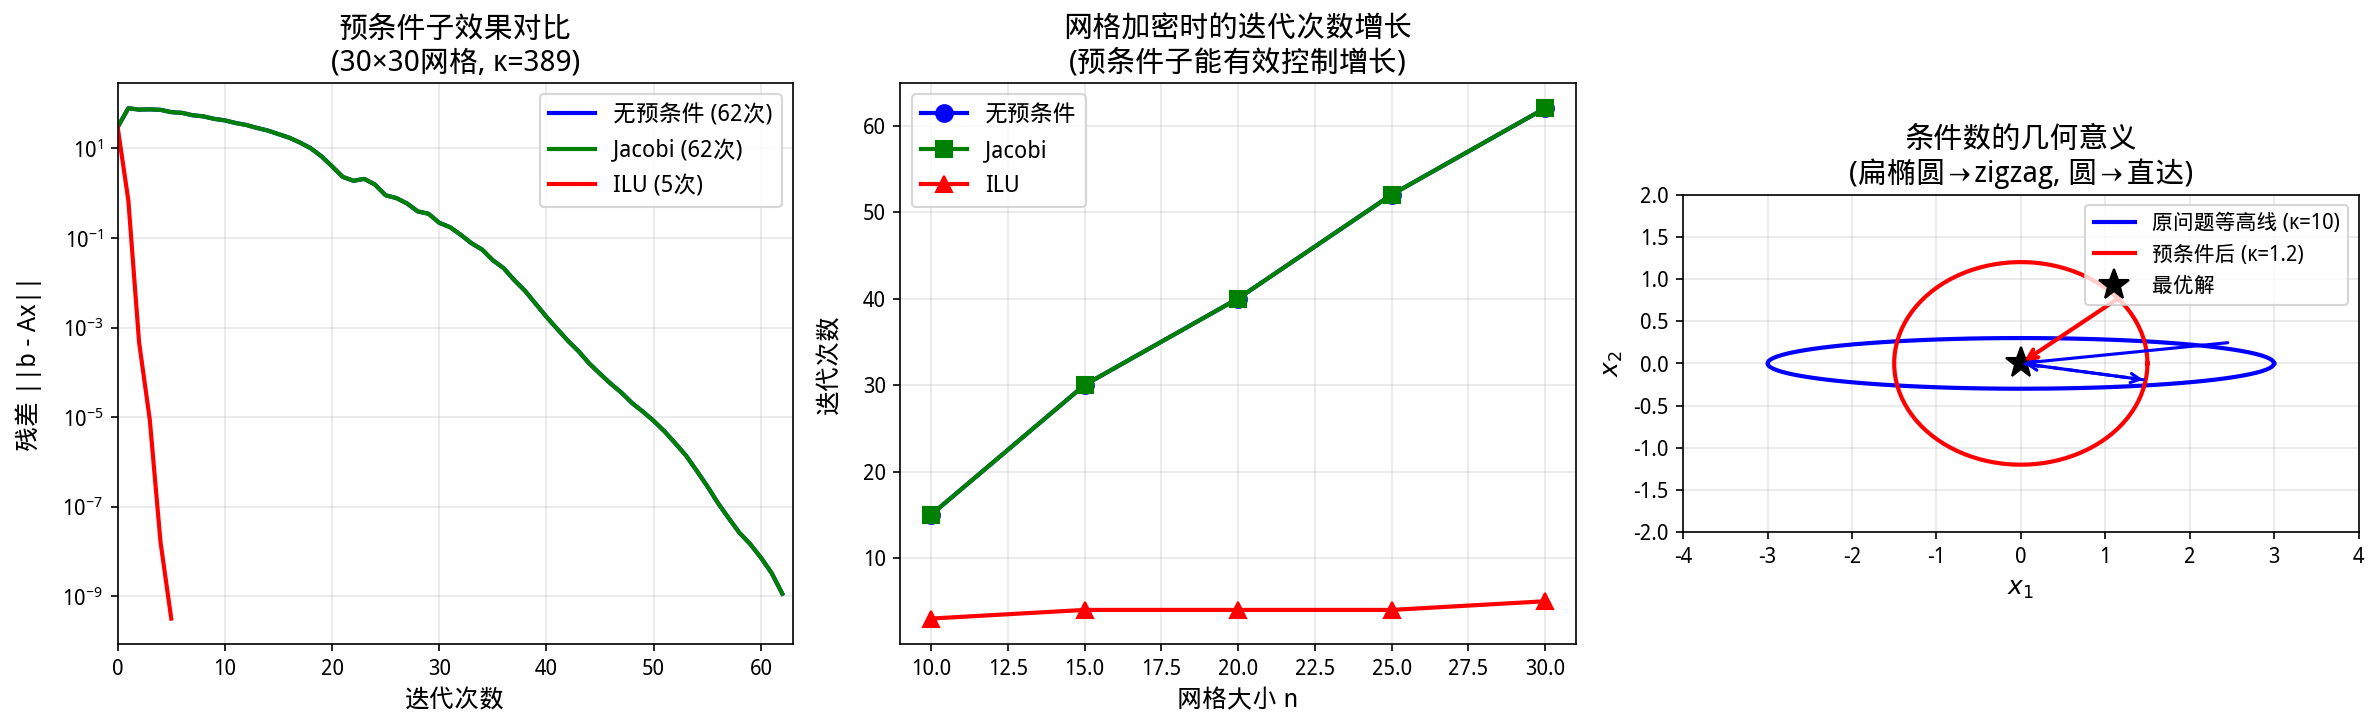
\includegraphics[width=0.95\textwidth]{figs_chap13/chap13_fig3.png}
\caption{预条件子效果的实验验证（1行3列）。\textbf{左图}：共轭梯度法收敛曲线对比——无预条件（蓝）、Jacobi预条件（绿）、ILU预条件（红），ILU只需约1/3的迭代次数；\textbf{中图}：网格加密时迭代次数的增长趋势——无预条件和Jacobi迭代次数线性增长，而ILU增长明显更慢；\textbf{右图}：条件数的几何意义——扁椭圆（高条件数）导致zigzag路径，圆形（低条件数）可以直达最优解。代码见 \texttt{code/chap05\_performance.py}。}
\label{fig:preconditioner}
\end{figure}

% ------------------------------------------------------------------------------------
\section*{CPU 并行计算的真正含义}
\addcontentsline{toc}{section}{CPU 并行计算的真正含义}

在学习数值计算和科学编程之前，初学者常常会问这样一个问题：

\begin{quote}
“为什么同样是一行代码，有的写法能快几十倍？为什么老师总让我用 NumPy，不要自己写循环？”
\end{quote}

要回答这个问题，我们必须从最基础的地方开始：CPU 是怎样执行程序的？它在什么情况下会变快、在什么情况下会变慢？这部分内容看似属于“计算机系统结构”，但它和我们写出高效代码息息相关。

为了让你真正“看得见”CPU 在做什么，我们会边讲概念边给出小实验。你可以在自己的电脑上立即验证这些现象，而不只是听一堆抽象的术语。

%==============================================================================
\subsection*{程序、进程与线程}
%==============================================================================

我们先从最核心的三个概念讲起。这三个词你可能早就听过，但很多人分不清它们的区别。

\paragraph{程序是什么？}

\textbf{程序（Program）}就是硬盘上的文件——一个 \verb|.exe|、一个 \verb|.py|、一个 \verb|.out|——本质上是一堆指令，静静地躺在那里，还没有执行。

打个比方：程序就像一本菜谱摆在书架上。你不动手做饭，它不会自己飘出味道来。

\paragraph{进程是什么？}

\textbf{进程（Process）}就是程序“开始执行”之后的样子。当你双击一个程序、或者在命令行输入 \verb|python xxx.py| 回车的那一刻，操作系统就会为这个程序创建一个进程。

进程最重要的特点是独立：它有自己独立的内存空间，别的进程看不到、也改不了；有自己的变量和数据结构；也有自己的一套运行状态。

继续用做饭来比喻：进程就是“你正在做菜”这件事本身。你占用了一整个厨房，锅、刀、案板、冰箱里的食材，都是你独占的。隔壁厨房在做什么菜，和你没关系。

\paragraph{线程是什么？}

\textbf{线程（Thread）}是进程内部的“执行路线”，或者说是“干活的小工”。一个进程可以同时雇好几个小工，让他们并行地帮你做事。

关键区别在于：同一个进程里的多个线程，\textbf{共享同一片内存空间}。它们可以直接读写同样的变量。

用厨房的比喻来说，一个进程是一家餐厅的厨房，线程是这个厨房里的多个厨师：厨师们共享同一个冰箱、同一套锅碗瓢盆（共享内存），但不同餐厅的厨房是完全隔开的（进程之间隔离）。

\begin{figure}[htbp]
\centering
\begin{tikzpicture}[scale=0.85]
    % 进程1
    \draw[thick, fill=blue!10, rounded corners] (0, 0) rectangle (5, 4);
    \node[font=\bfseries] at (2.5, 3.6) {进程 A（独立内存空间）};
    
    % 内存区域
    \draw[fill=yellow!20] (0.3, 2.2) rectangle (4.7, 3.2);
    \node[font=\small] at (2.5, 2.7) {共享内存：堆、全局变量};
    
    % A 的线程
    \foreach \x/\name in {0.5/线程1,2.1/线程2,3.7/线程3}{
        \draw[fill=green!30] (\x,0.5) rectangle ++(1.3,1.5);
        \node[font=\small, align=center] at (\x+0.65,1.25) {\name\\栈};
    }

    % 进程2
    \draw[thick, fill=red!10, rounded corners] (6, 0) rectangle (11, 4);
    \node[font=\bfseries] at (8.5, 3.6) {进程 B（独立内存空间）};
    \draw[fill=yellow!20] (6.3, 2.2) rectangle (10.7, 3.2);
    \node[font=\small] at (8.5, 2.7) {自己的内存};

    \foreach \x/\name in {6.5/线程1,8.2/线程2,9.9/线程3}{
        \draw[fill=orange!30] (\x,0.5) rectangle ++(1.3,1.5);
        \node[font=\small,align=center] at (\x+0.65,1.25) {\name\\栈};
    }

    % 隔离线
    \draw[ultra thick, red, dashed] (5.5,-0.5) -- (5.5,4.5);
    \node[red, font=\small] at (5.5,-0.8) {内存隔离};
\end{tikzpicture}
\caption{进程与线程的关系：进程之间相互隔离，而同一进程内的线程共享内存}
\end{figure}

下面这张表总结了进程和线程的主要区别：

\begin{center}
\small
\renewcommand{\arraystretch}{1.3}
\begin{tabularx}{\textwidth}{l|X|X}
\toprule
\textbf{特性} & \textbf{进程} & \textbf{线程} \\
\midrule
内存空间 & 独立，互不共享 & 共享同一进程的内存 \\
创建开销 & 较大（需申请整块内存） & 较小（主要是栈空间） \\
通信方式 & 需要特殊机制（管道、共享内存等） & 直接读写共享变量 \\
崩溃影响 & 一个进程挂了，其他不受影响 & 一个线程挂了，整个进程可能崩溃 \\
典型应用 & 浏览器的多个标签页 & 一个程序内部的并行计算 \\
\bottomrule
\end{tabularx}
\end{center}

%------------------------------------------------------------------------------
\paragraph{你可以自己做的小实验 1：Python 多线程为什么不快？}
%------------------------------------------------------------------------------

把下面的代码复制到你的电脑上运行一下：

\begin{lstlisting}[style=teaching, language=Python]
import threading
import time

def count():
    """一个简单的计数任务"""
    n = 0
    for _ in range(50_000_000):
        n += 1

# 先测试单线程
print("测试单线程...")
t0 = time.time()
count()
print(f"单线程耗时: {time.time() - t0:.2f} 秒")

# 再测试双线程
print("\n测试双线程...")
t0 = time.time()
t1 = threading.Thread(target=count)
t2 = threading.Thread(target=count)
t1.start()
t2.start()
t1.join()
t2.join()
print(f"双线程耗时: {time.time() - t0:.2f} 秒")
\end{lstlisting}

运行之后，你大概率会看到一个让人困惑的结果：单线程大约 2--3 秒，双线程却要 2--4 秒，甚至更慢。

这是怎么回事？开了两个线程，不是应该快一倍吗？

答案是：Python（准确说是 CPython 解释器）有一个特殊的设计叫 \textbf{GIL}（Global Interpreter Lock，全局解释器锁）。它规定：\textbf{同一时刻只能有一个线程在执行 Python 字节码}。

换句话说，即使你开了 10 个线程，Python 解释器也会让它们排队、轮流执行，而不是真正的并行。

这个实验让你亲眼看到了 GIL 的影响。后面我们会讲怎么绑过它。

%==============================================================================
\subsection*{内存层次与数据局部性}
%==============================================================================

当老师说“访问 L1 Cache 是 1 纳秒，访问主内存是 100 纳秒”的时候，初学者往往没有感觉。1 纳秒是什么？100 纳秒又是什么？快还是慢？

我们换一个更直观的比喻。

\sidenoteplain{
\textbf{小故事：}\\
1957 年，IBM 704 计算机的工程师们发现一个问题：CPU 算得太快，常常在“等”内存慢腾腾地把数据送过来。\\
于是他们在 CPU 旁边加了一小块极快的存储器，专门存最近用过的数据——这就是 Cache（高速缓存）的前身。\\
没想到，这个当年的“小补丁”后来成了所有现代处理器的标配设计。
}

想象一下你坐在办公桌前工作。\textbf{寄存器}（$<1$ ns）就像你手边的便签纸，伸手就能拿到；\textbf{L1 Cache}（$\sim 1$ ns）就像桌上的文件夹，抬手就能翻开；\textbf{L2/L3 Cache}（几 ns 到十几 ns）就像抽屉里的资料，需要弯腰去拿；\textbf{主内存 RAM}（$\sim 100$ ns）就像走去隔壁房间的档案柜取文件；\textbf{SSD 硬盘}（$\sim 100$ $\mu$s）则像开车去另一栋楼的仓库取东西。

现在你明白了吧？如果你的程序总是要“开车去仓库”，而别人的程序只需要“翻桌上的文件夹”，速度差别当然是天壤之别。

\begin{center}
\renewcommand{\arraystretch}{1.3}
\begin{tabular}{l|r|r|l}
\toprule
\textbf{层次} & \textbf{延迟（量级）} & \textbf{容量} & \textbf{类比} \\
\midrule
寄存器 & $< 1$ ns & 几十个字 & 手边的便签纸 \\
L1 Cache & $\sim 1$ ns & 32--64 KB & 桌上的文件夹 \\
L2/L3 Cache & 几--十几 ns & 数百 KB--数十 MB & 抽屉、柜子 \\
主内存（RAM） & $\sim 100$ ns & GB 级 & 隔壁房间档案室 \\
SSD & $\sim 100$ $\mu$s & TB 级 & 另一栋楼的仓库 \\
\bottomrule
\end{tabular}
\end{center}

这就引出了一个极其重要的概念：\textbf{数据局部性（Data Locality）}。

所谓数据局部性，就是说：如果你的程序访问的数据“挨在一起”，CPU 就能把它们一起搬进 Cache，后续访问就会非常快。反过来，如果你的程序东一下西一下地乱跳着访问数据，CPU 就不得不频繁地去“隔壁房间取文件”，速度就会慢很多。

%------------------------------------------------------------------------------
\paragraph{你可以自己做的小实验 2：按行访问 vs 按列访问}
%------------------------------------------------------------------------------

下面这个实验非常经典，能让你直观地“看见”Cache 的影响：

\begin{lstlisting}[style=teaching, language=Python]
import numpy as np
import time

N = 5000
A = np.random.rand(N, N)

# 方式一：按行访问（先固定 i，再遍历 j）
print("测试按行访问...")
t0 = time.time()
s = 0.0
for i in range(N):
    for j in range(N):
        s += A[i, j]
print(f"按行访问: {time.time() - t0:.2f} 秒")

# 方式二：按列访问（先固定 j，再遍历 i）
print("\n测试按列访问...")
t0 = time.time()
s = 0.0
for j in range(N):
    for i in range(N):
        s += A[i, j]
print(f"按列访问: {time.time() - t0:.2f} 秒")
\end{lstlisting}

运行之后，你会看到一个惊人的结果：按行访问大约 5--8 秒，按列访问却要 15--40 秒，慢了好几倍。

这两段代码做的事情完全一样——都是把矩阵所有元素加起来。循环次数也完全一样。为什么速度差这么多？

原因就在于 \textbf{NumPy 默认按行存储矩阵}（所谓 row-major order）。也就是说，\texttt{A[0,0]}, \texttt{A[0,1]}, \texttt{A[0,2]}, \ldots 这些元素在内存中是连续存放的。

当你按行访问时，CPU 读取 \texttt{A[0,0]} 的同时，会顺便把 \texttt{A[0,1]}, \texttt{A[0,2]}, \ldots 等一串数据都搬进 Cache。接下来你访问 \verb|A[0,1]| 时，它已经在 Cache 里了，不需要再去主内存取。

但当你按列访问时，你先访问 \verb|A[0,0]|，下一个却要访问 \verb|A[1,0]|——这两个数据在内存中相隔很远！CPU 刚搬进来的那一串数据全都用不上，又得重新去主内存取。这就是为什么按列访问会慢那么多。

\paragraph{结论：写数值代码时应该这样做}

写数值代码时，尽量让数据\textbf{连续存放}、按顺序访问（比如按行遍历矩阵），尽量\textbf{少做随机跳跃式}的访问；能在一次循环里完成的事情，就不要拆成好几个循环、每次都重新扫描整个大数组。

%==============================================================================
图~\ref{fig:chap13_python} 汇总了上面几个小实验的结果：多线程受 GIL 限制、按行访问快于按列访问、向量化远快于循环。下面逐一解释背后的原因。

\begin{figure}[htbp]
\centering
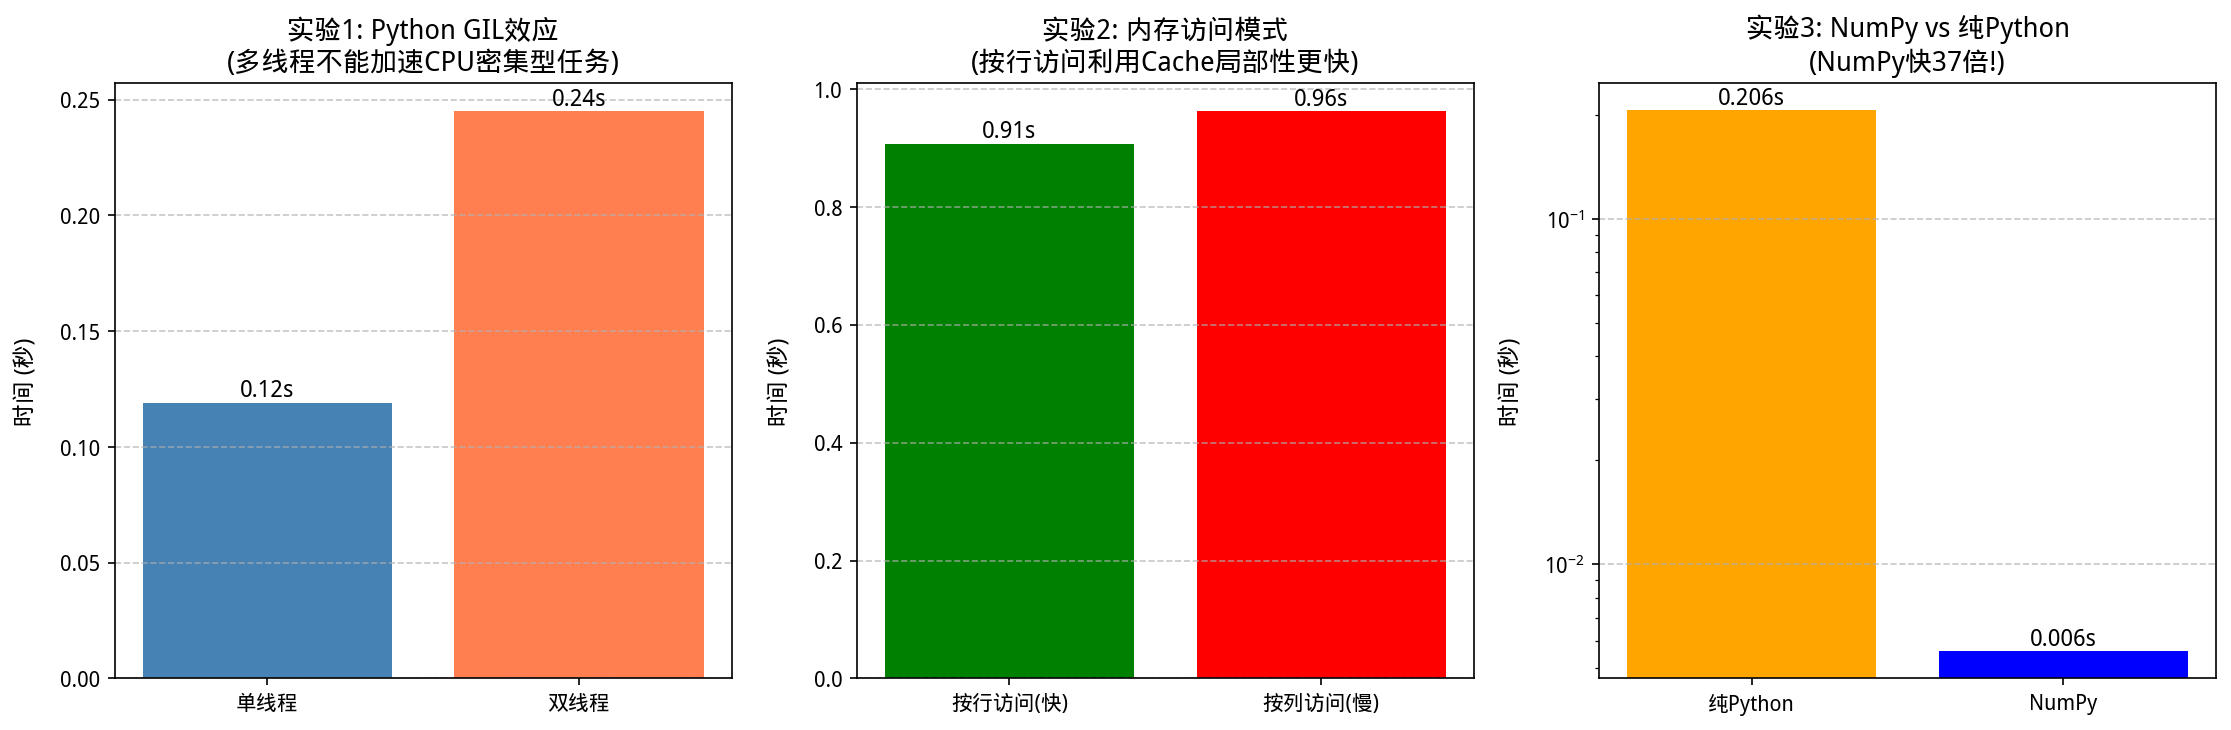
\includegraphics[width=0.95\textwidth]{figs_chap13/chap13_fig1.png}
\caption{Python性能优化实验：GIL对多线程的影响、缓存局部性的重要性、以及NumPy向量化的加速效果。左图显示Python多线程在CPU密集任务上受GIL限制，multiprocessing才能真正并行；中图展示行优先vs列优先遍历的性能差异（缓存局部性）；右图对比循环与向量化操作的速度——向量化可获得数十倍加速。}
\label{fig:chap13_python}
\end{figure}

\subsection*{Python 的 GIL：多线程为什么白忙活}
%==============================================================================

前面的实验已经让你看到了：Python 多线程在纯计算任务上并不能加速。现在我们来仔细解释一下原因。

\begin{definition}[全局解释器锁 GIL]
GIL（Global Interpreter Lock）是 CPython 解释器中的一个互斥锁。它的作用是：\textbf{保证同一时刻只有一个线程在执行 Python 字节码}。
\end{definition}

\begin{remark}
值得一提的是，Python 3.13（2024 年发布）开始提供“无 GIL”的实验性构建版本（称为 free-threaded 模式）。这意味着未来的 Python 有望真正支持多线程并行计算。不过，由于目前大多数生产环境和教学场景仍在使用 Python 3.10--3.12，而且许多第三方库尚未完全适配无 GIL 版本，本书仍以传统的带 GIL 的 Python 为基础进行讲解。当你阅读本书时，如果 Python 的无 GIL 版本已经成熟普及，下面关于“多线程无法加速计算密集型任务”的讨论可能就不再适用了——但理解 GIL 的历史和原理，仍然有助于你理解 Python 的设计哲学和大量遗留代码的行为。
\end{remark}

为什么 Python 要设计这么一个“奇怪”的锁呢？历史原因是：Python 的内存管理（特别是引用计数）不是线程安全的。如果允许多个线程同时修改 Python 对象，可能会导致内存错误。GIL 是一个简单粗暴但有效的解决方案。

GIL 的直接后果要分两种任务来看。对于 \textbf{IO 密集型任务}（比如网络请求、读写文件），多线程仍然有用，因为当一个线程在等待 IO 时，它会释放 GIL，让其他线程有机会执行。对于 \textbf{CPU 计算密集型任务}（比如大量数学运算），多线程基本没用，因为所有线程都在抢同一把锁、轮流执行，跟单线程没什么区别。

%------------------------------------------------------------------------------
\paragraph{那 Python 就没法并行计算了吗？}
%------------------------------------------------------------------------------

当然不是。有好几种方法可以绑过 GIL 的限制：

\begin{center}
\renewcommand{\arraystretch}{1.3}
\begin{tabular}{l|l|l}
\toprule
\textbf{方法} & \textbf{怎么做} & \textbf{适合什么场景} \\
\midrule
多进程 & 用 \verb|multiprocessing| 模块 & 计算密集型任务 \\
NumPy/SciPy & 调用底层 C/Fortran 库 & 数值计算（强烈推荐） \\
Numba/Cython & 把 Python 代码编译成机器码 & 热点代码加速 \\
异步 IO & 用 \verb|asyncio| 模块 & 网络、文件 IO \\
\bottomrule
\end{tabular}
\end{center}

对于初学者来说，最实用的建议是：\textbf{数值计算优先用 NumPy}，而不是自己写 Python 循环，因为 NumPy 的底层是 C 代码，不受 GIL 限制；如果确实需要用多核并行，就用 \verb|multiprocessing.Pool|：

\begin{lstlisting}[style=teaching, language=Python]
from multiprocessing import Pool
import time

def heavy_compute(x):
    """一个耗时的计算任务"""
    return sum(i * i for i in range(x))

if __name__ == "__main__":
    numbers = list(range(1000, 2000))
    
    # 单进程
    t0 = time.time()
    results1 = [heavy_compute(x) for x in numbers]
    print(f"单进程: {time.time() - t0:.2f} 秒")
    
    # 多进程（4 个工作进程）
    t0 = time.time()
    with Pool(processes=4) as pool:
        results2 = pool.map(heavy_compute, numbers)
    print(f"多进程: {time.time() - t0:.2f} 秒")
\end{lstlisting}

运行这段代码，你会发现多进程版本确实快了好几倍——因为每个进程有自己独立的 Python 解释器和 GIL，它们可以真正地并行执行。

%==============================================================================
\subsection*{NumPy 为什么比“纯 Python”快？}
%==============================================================================

很多老师会说：“\textbf{不要自己写 for 循环，尽量用 NumPy。}” 这句话背后的原因到底是什么？

主要有三条：

\paragraph{原因 1：底层是 C/Fortran 代码，没有解释器开销}

当你写一个 Python 循环时，解释器需要一行一行地“翻译”和执行。每一次循环迭代都有额外的开销：检查类型、查找变量、更新计数器……

\begin{lstlisting}[style=teaching, language=Python]
# 纯 Python：一百万次循环，解释器忙个不停
c = [a[i] + b[i] for i in range(1_000_000)]

# NumPy：一行代码，底层用 C 循环执行
c = a + b
\end{lstlisting}

第二行看起来很短，但它在底层做了很多事情：用 C 语言写的循环、没有 Python 解释器的开销、而且可以利用各种硬件优化。

\paragraph{原因 2：可以使用 SIMD 指令}

现代 CPU 有一类特殊的指令叫 SIMD（Single Instruction, Multiple Data）。顾名思义，一条指令可以同时处理多个数据。比如，一条 AVX 指令可以同时对 8 个浮点数做加法。

你在 Python 层面是看不到这些指令的，但 NumPy 底层的 C 代码会自动利用它们。

\paragraph{原因 3：底层库已经做好了多线程和 Cache 优化}

NumPy 的矩阵运算实际上调用的是 BLAS（Basic Linear Algebra Subprograms）库。这些库是几十年来无数专家精心优化的结晶：它们会自动把大矩阵分块，让每一块都能装进 Cache；会自动开多线程，用满 CPU 的所有核心；还针对不同的 CPU 架构做了专门优化。

%------------------------------------------------------------------------------
\paragraph{你可以自己做的小实验 3：感受 NumPy 的速度}
%------------------------------------------------------------------------------

\begin{lstlisting}[style=teaching, language=Python]
import numpy as np
import time

# 准备数据：500 万个随机数
x = np.random.rand(5_000_000)
y = np.random.rand(5_000_000)

# 方式一：纯 Python 循环
print("测试纯 Python...")
t0 = time.time()
z1 = [x[i] + y[i] for i in range(5_000_000)]
print(f"纯 Python: {time.time() - t0:.3f} 秒")

# 方式二：NumPy 向量运算
print("\n测试 NumPy...")
t0 = time.time()
z2 = x + y
print(f"NumPy: {time.time() - t0:.3f} 秒")
\end{lstlisting}

运行结果大概是：纯 Python 0.3--0.5 秒，NumPy 0.005--0.01 秒，快了\textbf{几十倍}，而且代码还更简洁。这就是为什么老师总让你用 NumPy。

\paragraph{对你来说最实用的一句总结}

如果你写的是数值计算代码，优先想一想：“\textbf{这个能不能写成 NumPy 的数组运算？}” 能用数组运算，就别写 Python 层的 for 循环。

%==============================================================================
\subsection*{CPU 与 GPU 的对比：不同的设计哲学}
%==============================================================================

最后，我们来简单聊聊 CPU 和 GPU 的区别。这个话题以后学深度学习时会深入讨论，这里先建立一个基本印象。

\paragraph{一句话总结}

\begin{quote}
CPU 是一个非常聪明的工人，能处理各种复杂任务。\\
GPU 是一大群比较简单的工人，但人多力量大。
\end{quote}

\paragraph{CPU 的设计哲学}

CPU 的核心数量不多（通常 4--64 个），但每个核心都非常强大：它有复杂的控制逻辑，能处理各种 if-else 分支；有乱序执行、分支预测等高级优化；还配有大容量的 Cache。所以 CPU 擅长处理流程复杂、分支很多、任务各不相同的程序，比如操作系统、编译器、数据库。

\paragraph{GPU 的设计哲学}

GPU 走的是另一条路：核心数量非常多（上千个），但每个核心都比较简单——只有简单的算术逻辑单元，擅长做加法、乘法，不擅长处理复杂的控制流；同时它有极高的内存带宽。所以 GPU 擅长处理“同一种运算要作用在大量数据上”的任务，比如矩阵乘法、图像处理、物理模拟。

\begin{center}
\renewcommand{\arraystretch}{1.3}
\begin{tabular}{l|l|l}
\toprule
\textbf{特性} & \textbf{CPU} & \textbf{GPU} \\
\midrule
核心数量 & 少（4--64） & 多（数千） \\
单核能力 & 强（复杂控制逻辑） & 弱（简单算术运算） \\
擅长任务 & 分支多、流程复杂 & 大规模并行计算 \\
内存带宽 & 较低 & 非常高 \\
编程难度 & 低 & 较高 \\
\bottomrule
\end{tabular}
\end{center}

%------------------------------------------------------------------------------
\paragraph{你可以自己做的小实验 4：CPU vs GPU 矩阵乘法}
%------------------------------------------------------------------------------

如果你的电脑有 NVIDIA 显卡，可以试试下面的代码（需要安装 PyTorch）：

\begin{lstlisting}[style=teaching, language=Python]
import torch
import time

# 准备两个大矩阵
A = torch.randn(4000, 4000)
B = torch.randn(4000, 4000)

# CPU 版本
print("测试 CPU...")
t0 = time.time()
C_cpu = A @ B
print(f"CPU: {time.time() - t0:.3f} 秒")

# GPU 版本（如果有 CUDA）
if torch.cuda.is_available():
    A_gpu = A.cuda()
    B_gpu = B.cuda()
    
    # 预热
    _ = A_gpu @ B_gpu
    torch.cuda.synchronize()
    
    print("\n测试 GPU...")
    t0 = time.time()
    C_gpu = A_gpu @ B_gpu
    torch.cuda.synchronize()
    print(f"GPU: {time.time() - t0:.3f} 秒")
else:
    print("\n（没有检测到 CUDA，跳过 GPU 测试）")
\end{lstlisting}

如果你有 GPU，会看到类似这样的结果：CPU 需要 1--3 秒，GPU 只要 0.01--0.05 秒，快了\textbf{几十倍到上百倍}。这就是为什么深度学习训练几乎都在 GPU 上进行。

%==============================================================================
\subsection*{并行计算的层次结构}
%==============================================================================

到这里，我们可以把并行计算的各种层次整理一下：

\begin{figure}[htbp]
\centering
\begin{tikzpicture}[
    box/.style={draw, rounded corners, minimum width=4.5cm, minimum height=0.9cm, font=\small, align=center},
    scale=0.95
]
    \node[box, fill=red!20] at (0, 4.5) {指令级并行（ILP）\\CPU 硬件自动完成};
    \node[box, fill=orange!20] at (0, 3.0) {数据级并行（SIMD）\\NumPy、向量指令};
    \node[box, fill=yellow!20] at (0, 1.5) {线程/进程级并行\\多线程、多进程};
    \node[box, fill=green!20] at (0, 0) {节点级并行\\多机集群、MPI};
    
    \draw[<->, thick] (-3.2, -0.3) -- (-3.2, 4.8);
    \node[left, font=\small, rotate=90] at (-3.5, 2.25) {粒度：从细到粗};
    
    \draw[<->, thick] (3.2, -0.3) -- (3.2, 4.8);
    \node[right, font=\small, rotate=270] at (3.5, 2.25) {编程难度：从低到高};
\end{tikzpicture}
\caption{并行计算的层次：越往上粒度越细，通常由硬件或编译器自动完成；越往下粒度越粗，需要程序员手动管理}
\end{figure}

对于初学者来说，这四层里真正要操心的很少：\textbf{指令级并行}你不需要管，CPU 会自动做；\textbf{数据级并行}用 NumPy 就能享受到，不需要自己写；\textbf{线程/进程级并行}需要时可以用 \verb|multiprocessing|；\textbf{节点级并行}等你以后做大规模计算再学。

%==============================================================================
\subsection*{本节小结：给你的实践建议}
%==============================================================================

第一次接触这些概念的读者，应该记住以下几点：

\begin{enumerate}
    \item \textbf{写数值代码时，优先用 NumPy}，而不是纯 Python 循环。这一条最重要。
    
    \item \textbf{注意数据的访问模式}。尽量让数据连续存放、按顺序访问。避免随机跳跃式的访问。
    
    \item \textbf{Python 多线程对 CPU 密集型任务没用}，因为 GIL 的存在。需要多核并行时，用多进程。
    
    \item \textbf{当程序变慢时}，不要第一反应怪“电脑太差”。先想想：是不是在用 Python 循环遍历大数组？是不是内存访问模式很“跳跃”？是不是开了很多线程但被 GIL 卡住？
    
    \item \textbf{GPU 适合大规模并行计算}（比如矩阵运算），CPU 适合复杂逻辑。以后遇到“同一种计算要做几百万次”的任务，就可以考虑用 GPU。
\end{enumerate}

掌握这些基础概念，你以后再学操作系统、计算机体系结构、并行计算课程时会轻松很多。而且从现在开始，你就可以写出\textbf{更快、更高效}的数值计算代码了。


% ====================================================================================
\section*{流固耦合有限元：Turek--Hron 基准}
\addcontentsline{toc}{section}{流固耦合有限元：Turek--Hron 基准}
% ====================================================================================

\begin{tcolorbox}[colback=gray!5, colframe=gray!50, title=本节导读]
你有没有见过大风中摇晃的旗杆？或者听说过塔科马海峡大桥在风中剧烈扭曲最终坍塌的故事？

这些现象背后有一个共同的物理机制：\textbf{流固耦合}（Fluid-Structure Interaction, FSI）。流体（空气或水）作用于固体结构，固体的变形又反过来影响流场，形成复杂的相互作用。

本节介绍流固耦合领域最著名的基准测试——\textbf{Turek-Hron FSI2问题}：一个弹性薄板固连在圆柱后方，在来流作用下发生大幅度自激振荡。这个问题展示了涡激振动的典型特征，也是验证FSI求解器的工业标准。
\end{tcolorbox}

% ------------------------------------------------------------------------------------
\subsection*{一、问题描述：圆柱后的弹性旗}

Turek和Hron在2006年提出了一系列FSI基准测试问题，其中\textbf{FSI2}是最具挑战性也最常被引用的一个。

\begin{figure}[htbp]
\centering
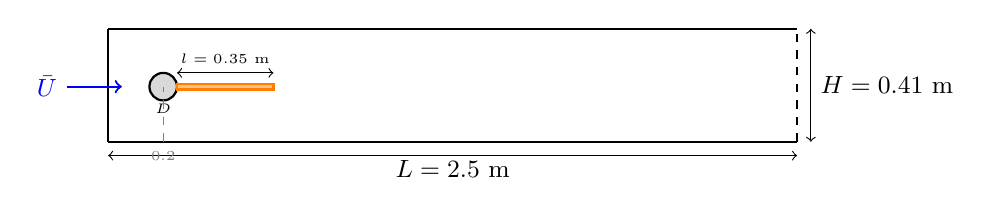
\begin{tikzpicture}[scale=3.5]
    % 通道
    \draw[thick] (0,0) -- (2.5,0);
    \draw[thick] (0,0.41) -- (2.5,0.41);

    % 入口
    \draw[thick] (0,0) -- (0,0.41);
    \draw[->, blue, thick] (-0.15,0.2) -- (0.05,0.2);
    \node[blue, left] at (-0.15,0.2) {\small $\bar{U}$};

    % 出口
    \draw[thick, dashed] (2.5,0) -- (2.5,0.41);

    % 圆柱
    \fill[gray!30] (0.2,0.2) circle (0.05);
    \draw[thick] (0.2,0.2) circle (0.05);
    \node at (0.2,0.12) {\tiny $D$};

    % 弹性板
    \fill[orange!50] (0.25,0.19) rectangle (0.6,0.21);
    \draw[thick, orange] (0.25,0.19) -- (0.6,0.19) -- (0.6,0.21) -- (0.25,0.21) -- cycle;

    % 标注
    \draw[<->] (0,-0.05) -- (2.5,-0.05);
    \node at (1.25,-0.1) {\small $L = 2.5$ m};
    \draw[<->] (2.55,0) -- (2.55,0.41);
    \node[right] at (2.55,0.205) {\small $H = 0.41$ m};

    % 板的标注
    \draw[<->] (0.25,0.25) -- (0.6,0.25);
    \node[above] at (0.425,0.25) {\tiny $l = 0.35$ m};

    % 圆心位置
    \draw[dashed, gray] (0.2,0) -- (0.2,0.2);
    \node[gray, below] at (0.2,0) {\tiny 0.2};
\end{tikzpicture}
\caption{Turek-Hron FSI2几何设置。矩形通道（$2.5 \times 0.41$ m）内有一刚性圆柱（直径$D = 0.1$ m），圆心在$(0.2, 0.2)$m处（故意偏心以打破对称性）。一块弹性薄板（长$0.35$ m，厚$0.02$ m，橙色）固连在圆柱后方。流体从左侧入口以抛物线速度剖面进入。}
\label{fig:turek_fsi_geometry}
\end{figure}

\paragraph{物理参数}

\begin{center}
\renewcommand{\arraystretch}{1.3}
\begin{tabular}{l|l|l}
\toprule
\textbf{参数} & \textbf{符号} & \textbf{FSI2取值} \\
\midrule
流体密度 & $\rho_f$ & 1000 kg/m³ \\
动力粘度 & $\mu_f$ & 0.001 Pa$\cdot$s \\
平均入口速度 & $\bar{U}$ & 1.0 m/s \\
雷诺数 & Re $= \rho_f \bar{U} D / \mu_f$ & 100 \\
\midrule
固体密度 & $\rho_s$ & 10000 kg/m³ \\
杨氏模量 & $E$ & $1.4 \times 10^6$ Pa \\
泊松比 & $\nu_s$ & 0.4 \\
\midrule
密度比 & $\rho_s / \rho_f$ & 10 \\
\bottomrule
\end{tabular}
\end{center}

\sidenoteplain{\textbf{为什么圆心偏心？} 如果圆柱在通道正中央，由于对称性，初始阶段不会产生涡脱落。偏心打破了对称性，使得流动从一开始就不稳定，更快进入周期性振荡状态。}

% ------------------------------------------------------------------------------------
\subsection*{二、涡激振动机理}

当流体绕过圆柱时，会在圆柱两侧交替脱落旋转方向相反的涡——这就是著名的\textbf{卡门涡街}（Kármán vortex street）。

\sidenoteplain{\textbf{西奥多·冯·卡门}（Theodore von Kármán, 1881--1963）是20世纪最伟大的航空工程师之一。他不仅发现了卡门涡街，还创立了喷气推进实验室（JPL），培养了钱学森等众多杰出学生。}

\begin{figure}[htbp]
\centering
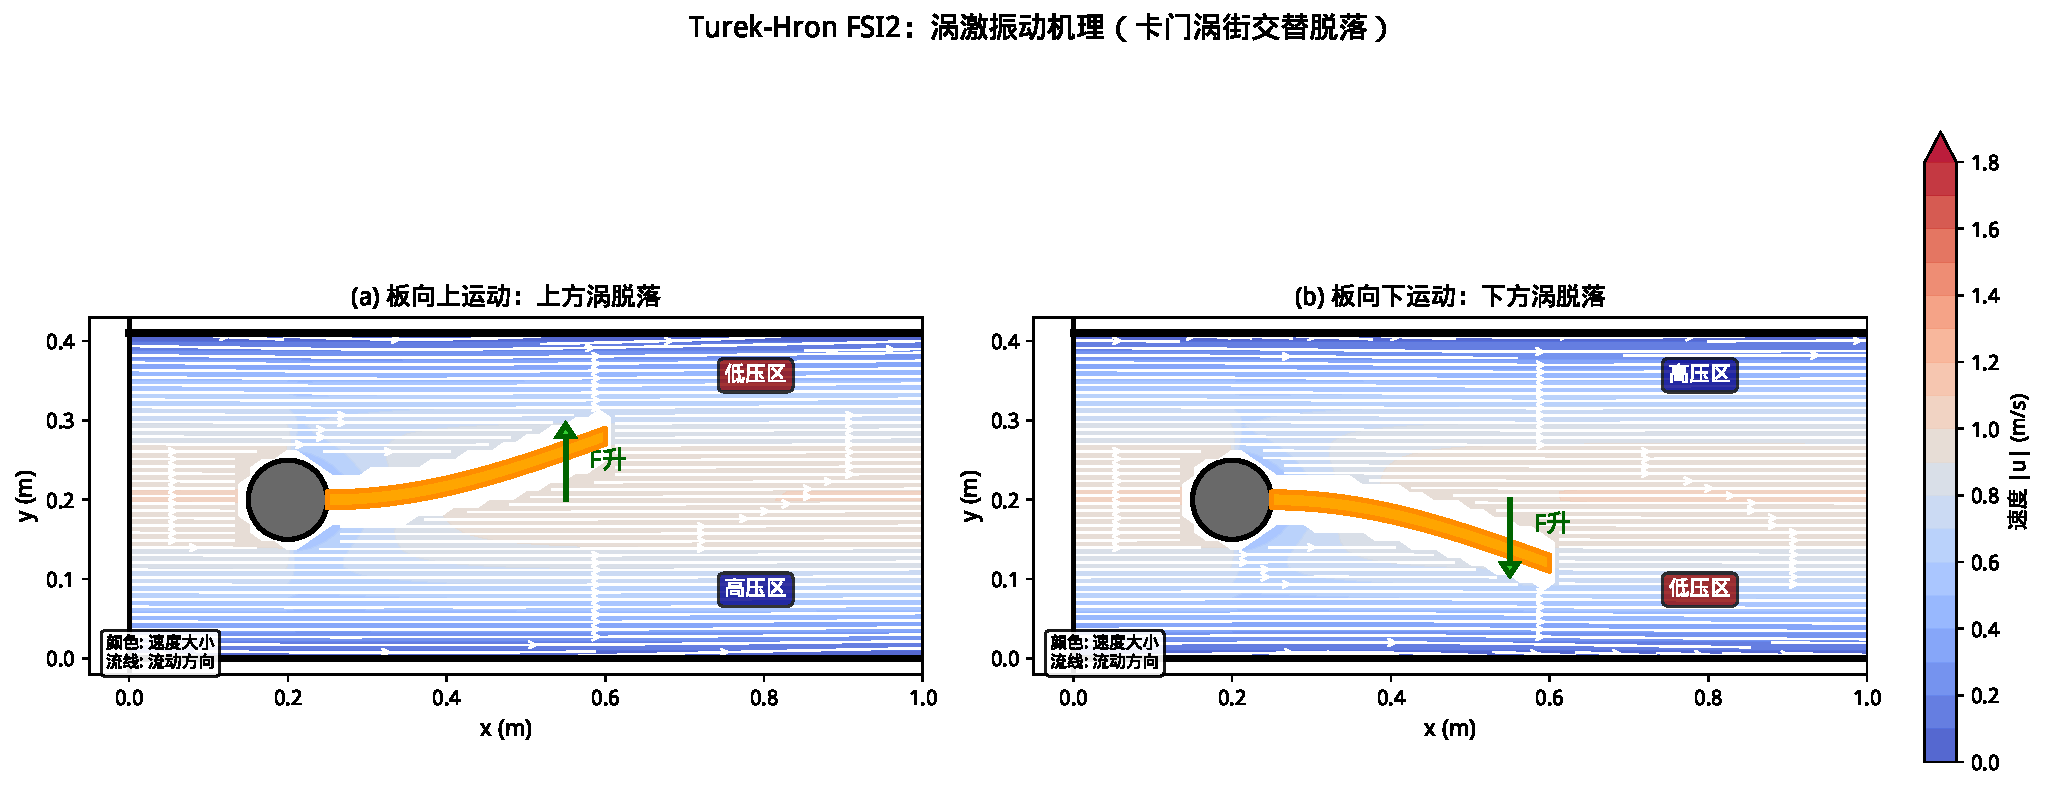
\includegraphics[width=0.98\textwidth]{figs_chap13/turek_fsi2_mechanism.pdf}
\caption{涡激振动机理示意。(a) 当上方涡脱落时，圆柱和板上方形成低压区，产生向上的升力，推动弹性板向上弯曲。(b) 半个周期后，下方涡脱落，下方形成低压区，产生向下的升力。这种交替的压力差驱动板的周期性振荡。}
\label{fig:turek_fsi2_mechanism}
\end{figure}

涡脱落频率由\textbf{Strouhal数}确定：
\begin{equation}
f_s = \text{St} \cdot \frac{U}{D}
\end{equation}
其中$\text{St} \approx 0.2$对于许多钝体都近似成立。对于FSI2条件：$f_s \approx 0.2 \times 1.0 / 0.1 = 2$ Hz。

当这个涡脱落频率接近弹性板的固有频率时，会发生\textbf{锁定}（lock-in）现象：涡脱落频率被“锁定”到结构固有频率上，振幅急剧增大，流固相互作用形成正反馈，系统进入\textbf{自激振荡}。

% ------------------------------------------------------------------------------------
\subsection*{三、振动响应}

经过初始瞬态后，弹性板进入稳态周期振荡。图\ref{fig:turek_fsi2_snapshots}展示了一个振动周期内弹性板的变形序列。

\begin{figure}[htbp]
\centering
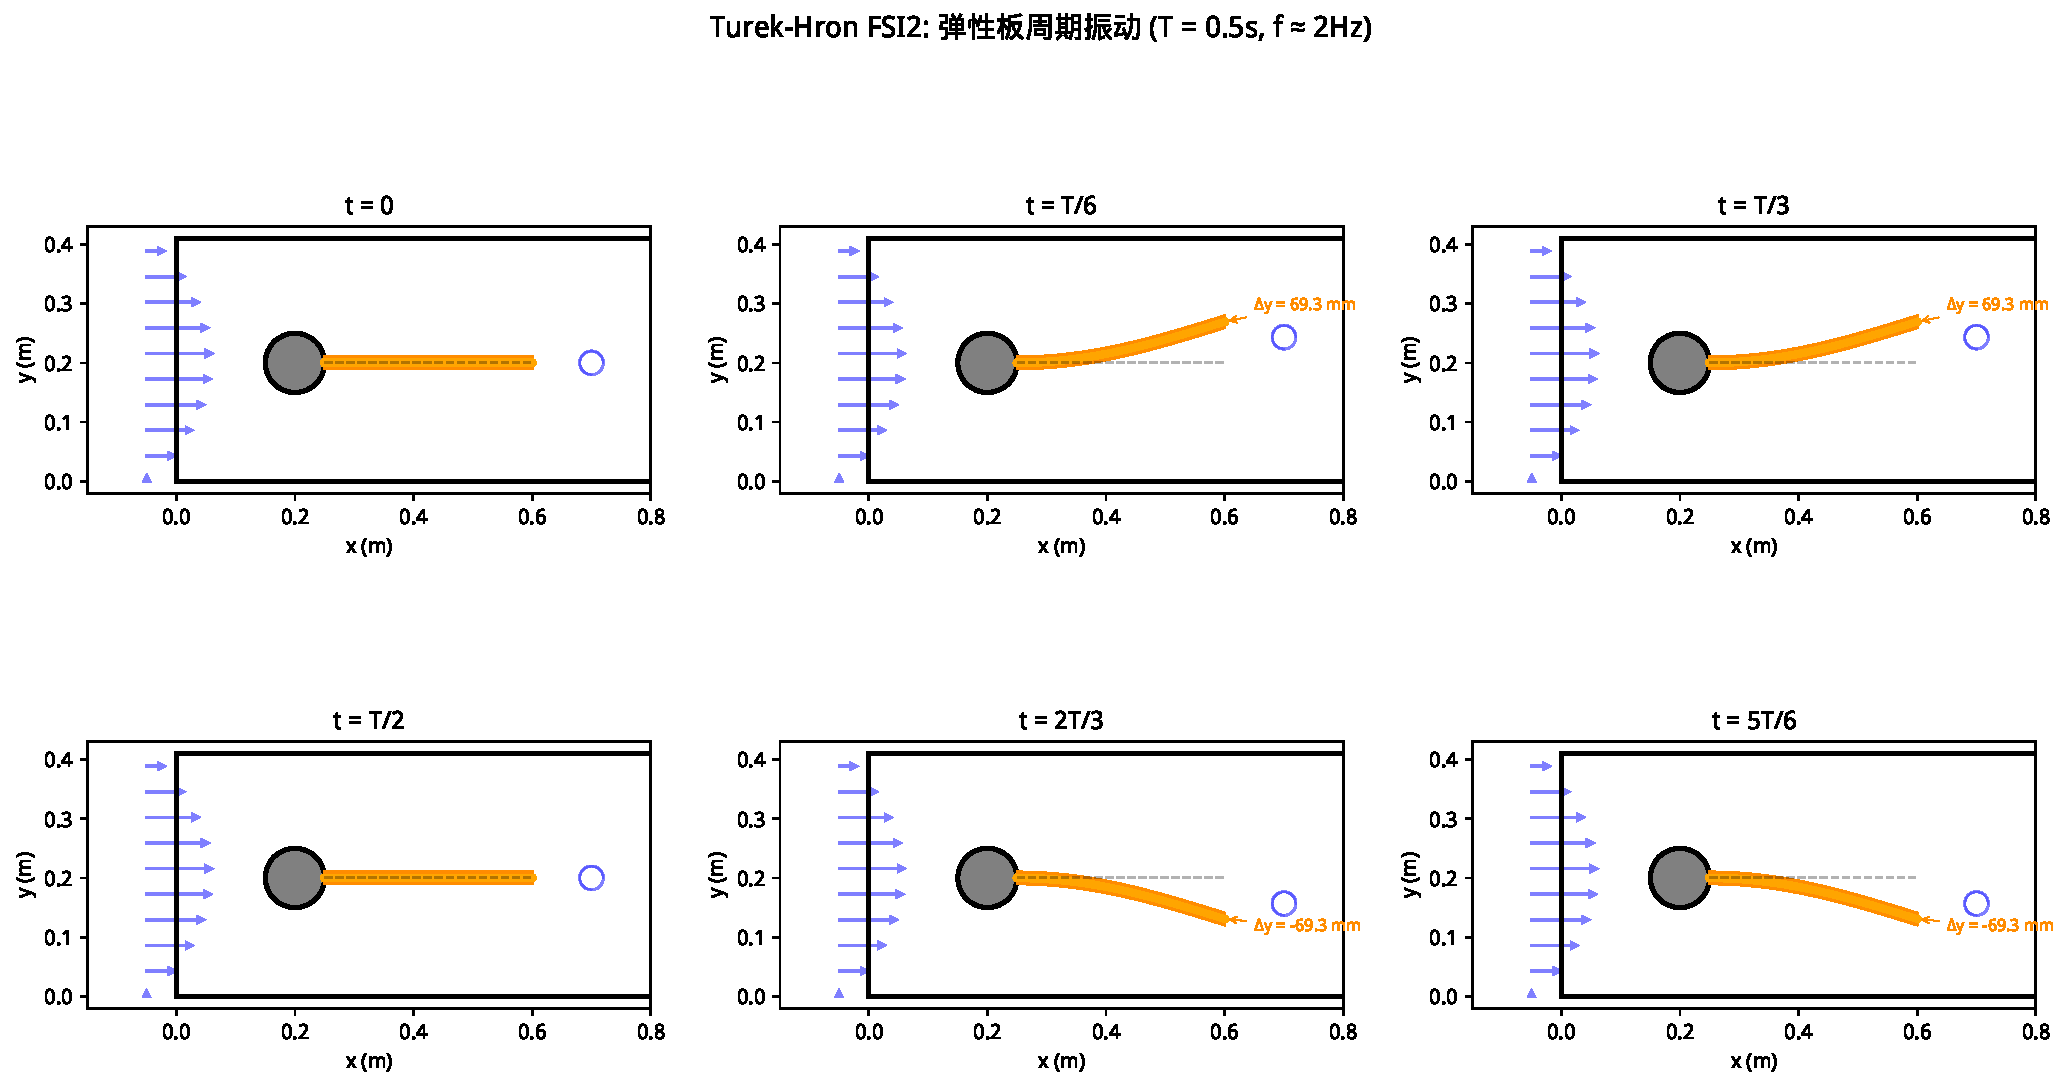
\includegraphics[width=0.98\textwidth]{figs_chap13/turek_fsi2_snapshots.pdf}
\caption{Turek-Hron FSI2：弹性板在一个振动周期（$T \approx 0.5$ s）内的变形快照。板端Y方向位移幅值约$\pm 80$ mm，这是板长（350 mm）的约23\%——属于大变形范畴！注意板的变形主要由一阶弯曲模态主导。}
\label{fig:turek_fsi2_snapshots}
\end{figure}

图\ref{fig:turek_fsi2_analysis}给出了完整的动力学分析。

\begin{figure}[htbp]
\centering
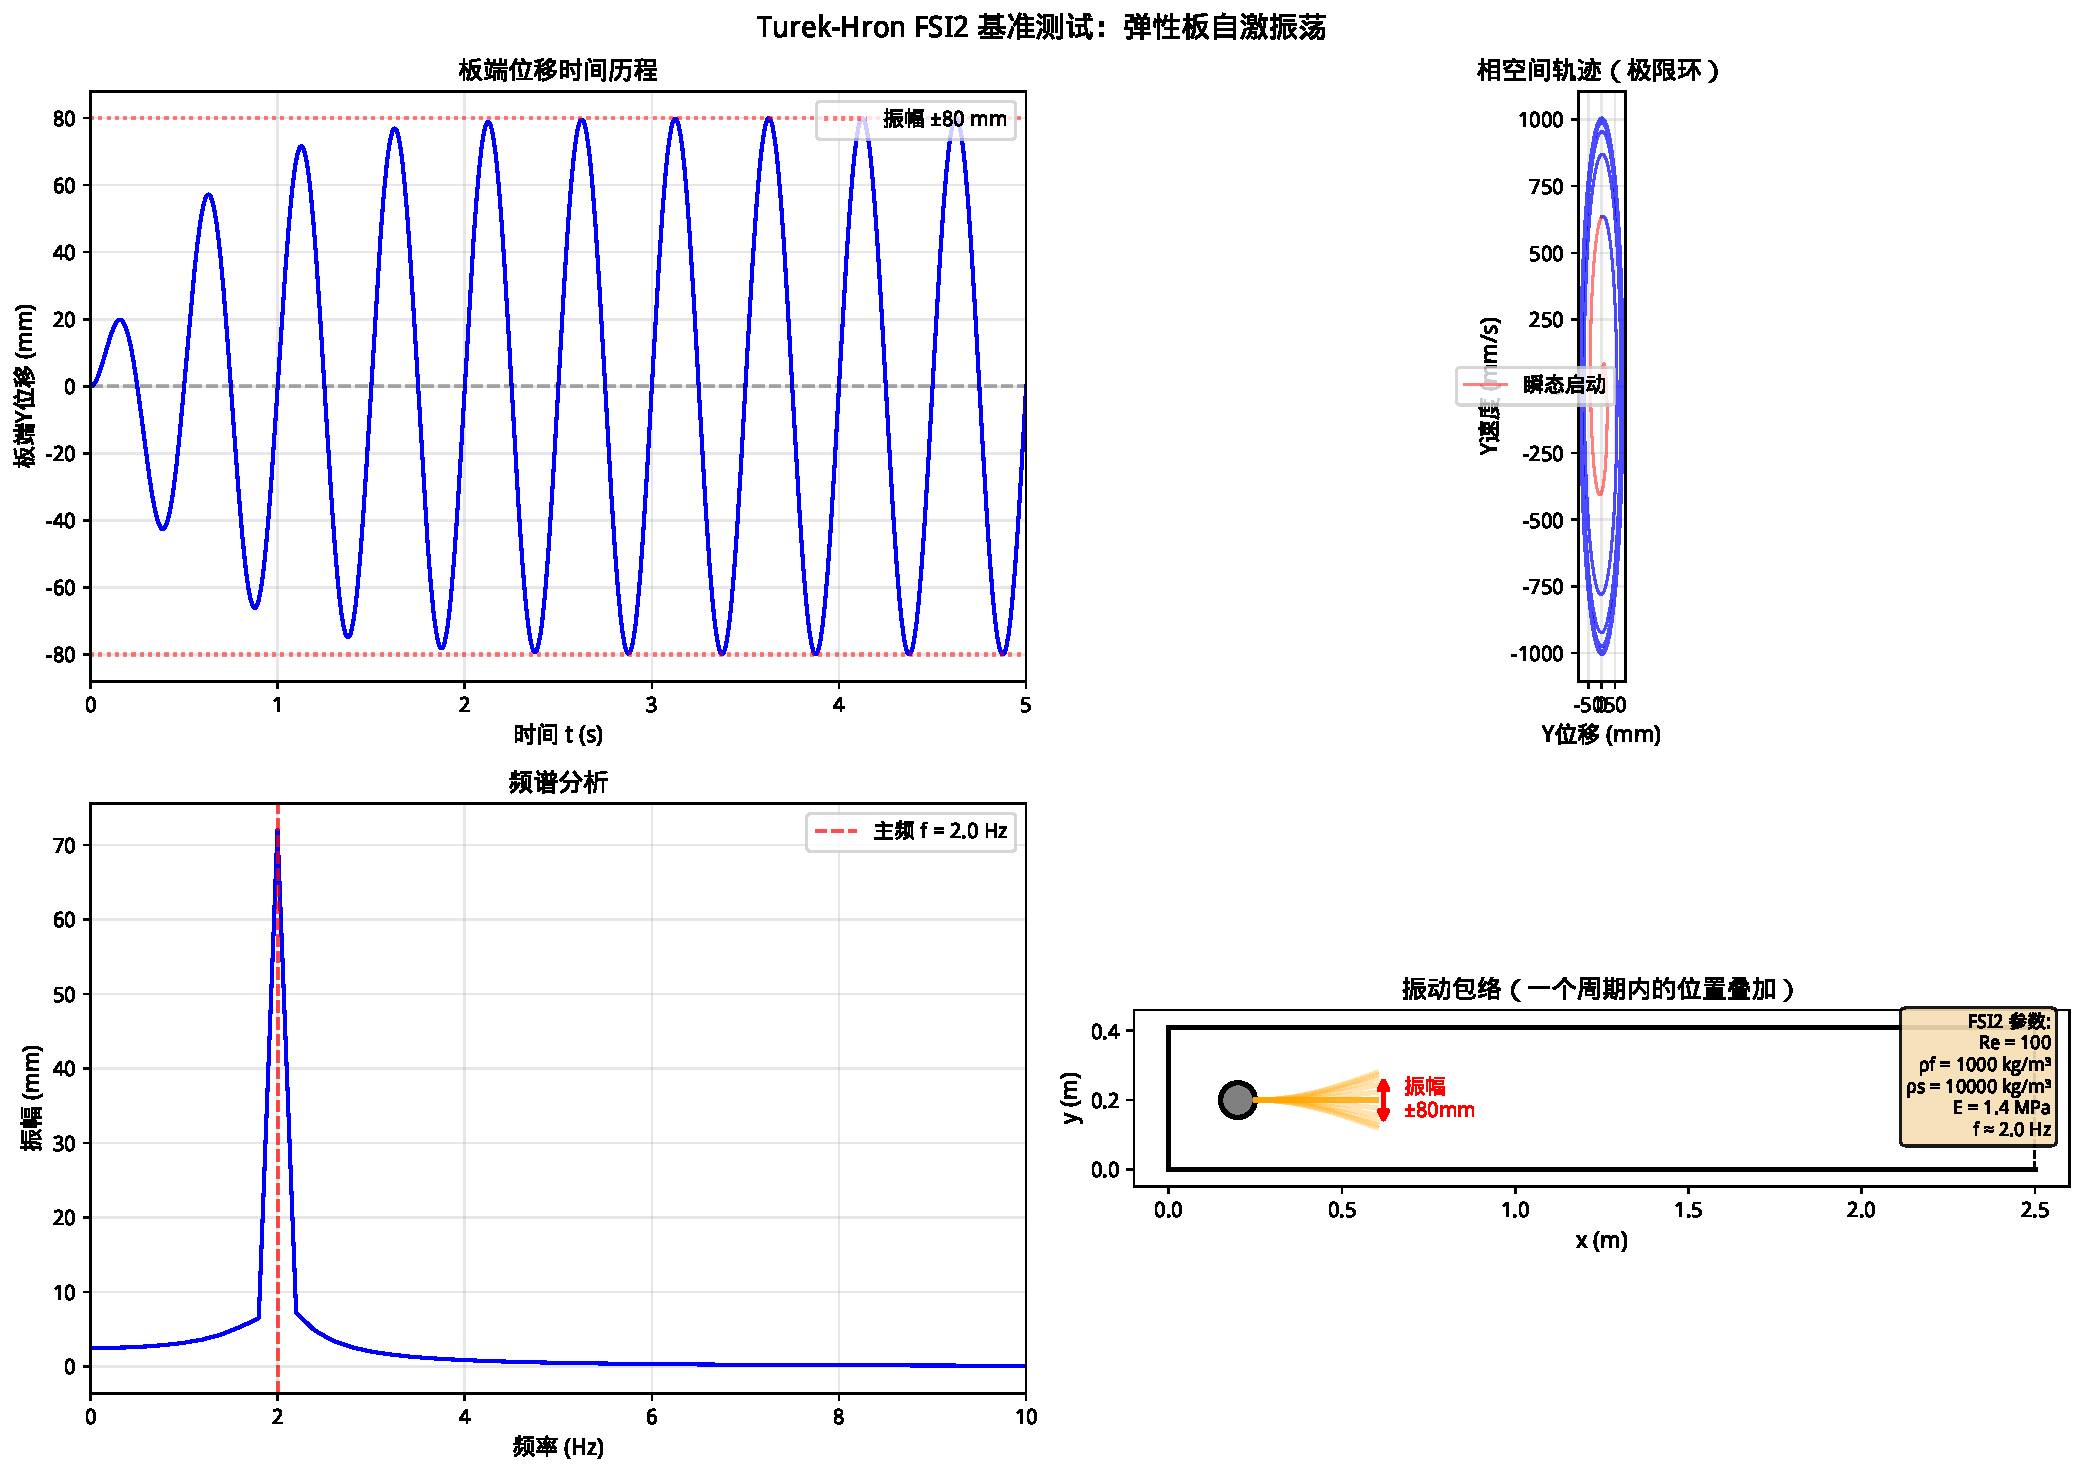
\includegraphics[width=0.98\textwidth]{figs_chap13/turek_fsi2_time_history.pdf}
\caption{Turek-Hron FSI2动力学分析。\textbf{左上}：板端Y位移时间历程——经过短暂瞬态后进入稳态振荡，振幅约$\pm 80$ mm。\textbf{右上}：相空间轨迹——稳态时形成极限环（limit cycle），这是自激振荡的标志。\textbf{左下}：频谱分析——主频约2 Hz，与涡脱落频率一致。\textbf{右下}：振动包络——一个周期内板的位置叠加，展示振动的空间范围。}
\label{fig:turek_fsi2_analysis}
\end{figure}

图\ref{fig:turek_fsi2_vortex_street}展示了涡街演化与固体振动的耦合过程，清晰可见卡门涡街的交替脱落如何驱动弹性板的周期性摆动。

\begin{figure}[htbp]
\centering
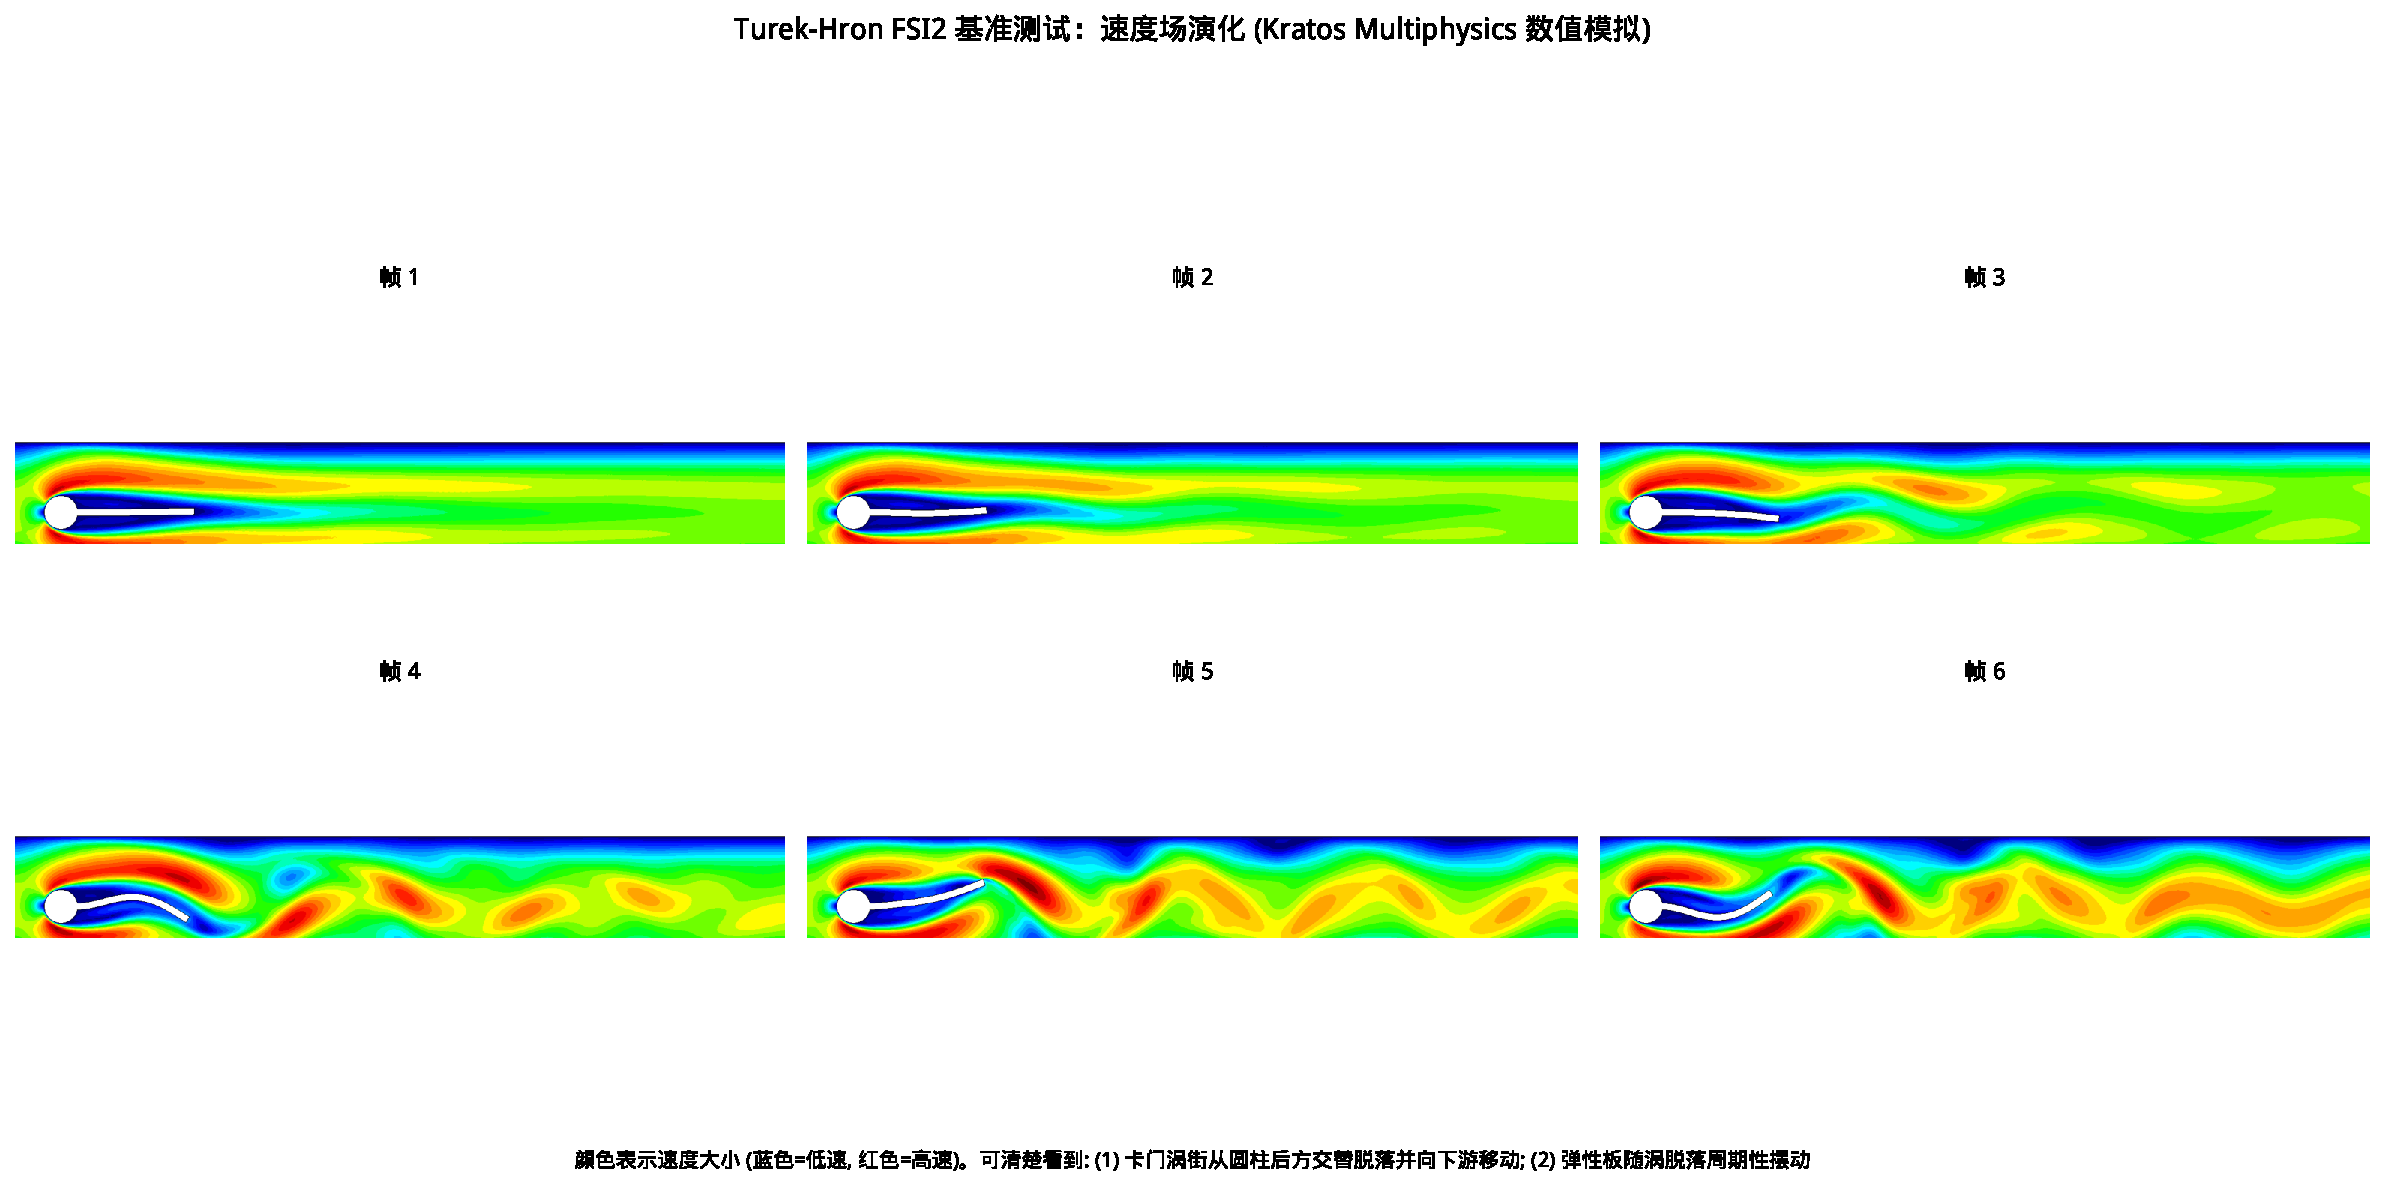
\includegraphics[width=0.98\textwidth]{figs_chap13/turek_fsi2_cfd_velocity.pdf}
\caption{Turek-Hron FSI2基准测试的CFD模拟结果（Kratos Multiphysics开源软件）。颜色表示流体速度大小（蓝色=低速，红色=高速）。可以清楚看到：(1) 卡门涡街从圆柱后方交替脱落并向下游对流移动；(2) 弹性板（白色）随着涡的周期性脱落发生大幅度弯曲振荡；(3) 流场呈现典型的涡激振动特征，高速区（红/橙色）和低速区（蓝色）交替出现。}
\label{fig:turek_fsi2_vortex_street}
\end{figure}

\paragraph{文献参考值}
Turek 和 Hron 报告的 FSI2 基准结果是：板端 Y 方向位移 $y(A) = (1.23 \pm 80.6) \times 10^{-3}$ m，即均值 1.23 mm、振幅 80.6 mm；振动频率 $f \approx 2.0$ Hz；圆柱阻力系数 $C_D = 208.83 \pm 73.75$，升力系数 $C_L = 0.88 \pm 234.2$。

% ------------------------------------------------------------------------------------
\subsection*{四、结构建模：Euler--Bernoulli 梁}

弹性板可以用\textbf{Euler-Bernoulli梁理论}建模。控制方程为：
\begin{equation}
EI \frac{\partial^4 w}{\partial x^4} + \rho A \frac{\partial^2 w}{\partial t^2} = f(x, t)
\end{equation}
其中$w(x,t)$是横向位移，$EI$是抗弯刚度，$\rho A$是单位长度质量，$f(x,t)$是流体力。

\subsubsection*{单元刚度矩阵与质量矩阵}

对于长度为$L_e$的梁单元，每端有两个自由度（位移$w$和转角$\theta$），单元矩阵是$4 \times 4$的：
\begin{align}
\mathbf{K}_e &= \frac{EI}{L_e^3}
\begin{pmatrix}
12 & 6L_e & -12 & 6L_e \\
6L_e & 4L_e^2 & -6L_e & 2L_e^2 \\
-12 & -6L_e & 12 & -6L_e \\
6L_e & 2L_e^2 & -6L_e & 4L_e^2
\end{pmatrix}, \\
\mathbf{M}_e &= \frac{\rho A L_e}{420}
\begin{pmatrix}
156 & 22L_e & 54 & -13L_e \\
22L_e & 4L_e^2 & 13L_e & -3L_e^2 \\
54 & 13L_e & 156 & -22L_e \\
-13L_e & -3L_e^2 & -22L_e & 4L_e^2
\end{pmatrix}
\end{align}

\sidenoteplain{\textbf{注意}：FSI2涉及大变形，严格来说需要使用几何非线性公式（如协同旋转法或Total Lagrangian公式）。这里的线性梁模型只是演示目的。}

% ------------------------------------------------------------------------------------
\subsection*{五、完整FSI求解的挑战}

Turek-Hron FSI2之所以成为经典基准，是因为它包含了FSI问题的核心难点：

\begin{insightbox}
\textbf{FSI2 的挑战}：板端位移约 80 mm，是板长的 23\%，几何非线性显著，这是\textbf{大变形}；密度比 $\rho_s/\rho_f = 10$ 适中，流固相互作用强烈，这是\textbf{强耦合}；振荡不是外加的强迫振动，而是系统自发产生的不稳定性，这是\textbf{自激振荡}；结构变形影响流场，流场变化又反馈到结构力，这是\textbf{双向耦合}。
\end{insightbox}

完整求解 FSI2 需要同时求解三部分。\textbf{流体}一侧是不可压缩 Navier--Stokes 方程
\begin{equation}
\rho_f \left( \frac{\partial \mathbf{v}}{\partial t} + \mathbf{v} \cdot \nabla \mathbf{v} \right) = -\nabla p + \mu_f \nabla^2 \mathbf{v} ;
\end{equation}
\textbf{固体}一侧是非线性弹性动力学方程（Saint-Venant--Kirchhoff 材料）；两者通过流固界面上的\textbf{耦合条件}——速度连续、应力平衡——连在一起。这需要迭代求解或整体求解，计算成本比单独的流体或结构问题高 1--2 个数量级。

% ------------------------------------------------------------------------------------
\subsection*{六、开源实现}

\sidenoteplain{\textbf{开源FSI框架}：Kratos Multiphysics（完整的多物理场框架）、preCICE（连接不同求解器的耦合库）、Feel++（C++ FEM 库）、oomph-lib（牛津大学开发的多物理场库），以及 OpenFOAM + CalculiX 的流体+结构组合，都包含 Turek--Hron 基准案例的实现。}

本节的示意图由 \texttt{code\_chap13} 目录下的 Python 脚本 \texttt{turek\_fsi2\_\allowbreak visualization.py} 生成；真正的 FSI2 求解需要使用专业的多物理场软件。

\begin{lstlisting}[language=Python, caption=弹性板变形计算示意]
def flag_deformation(s, t, amplitude=0.080, freq=2.0):
    """
    计算弹性板在给定时刻的变形
    s: 沿板长度的参数 [0, 1], 0=固定端, 1=自由端
    t: 时间
    """
    # 一阶弯曲模态: phi(s) ~ 1 - cos(pi*s/2)
    phi = 1 - np.cos(np.pi * s / 2)
    omega = 2 * np.pi * freq
    y_displacement = amplitude * phi * np.sin(omega * t)
    return y_displacement
\end{lstlisting}

% ------------------------------------------------------------------------------------
\subsection*{七、工程意义}

涡激振动不仅是学术问题，在工程中有重大实际意义。海洋工程里，深海立管（riser）在洋流中的涡激振动是设计的主要挑战；桥梁工程里，塔科马海峡大桥（1940 年坍塌）的前期振动就与涡激振动有关；航空航天里有飞机机翼、尾翼的气动弹性颤振；能源工程里则有风力机叶片、热交换器管束的振动。

\sidenoteplain{\textbf{塔科马海峡大桥}（1940年坍塌）长期被误解为共振导致。现代分析表明，真正原因是\textbf{气动弹性颤振}——一种更复杂的流固耦合不稳定性。但涡激振动确实是该桥在坍塌前频繁振动的重要原因。}

\begin{insightbox}
\textbf{为什么 Turek--Hron 基准如此重要？}前面说的大变形、强耦合与自激振荡三个难点，足以考验一个 FSI 求解器；而作为纯数值基准，它还有一个实验无法提供的优点——\textbf{无实验噪声}，可以进行严格的代码间比较。
\end{insightbox}

如果你的FSI代码能正确重现Turek-Hron基准的结果，那它就有了一定的可信度。这就是为什么FSI2成为了验证FSI求解器的“金标准”。

\paragraph{本节参考文献}
\begin{enumerate}
    \item S. Turek and J. Hron, ``Proposal for Numerical Benchmarking of Fluid-Structure Interaction between an Elastic Object and Laminar Incompressible Flow,'' in \textit{Fluid-Structure Interaction}, Lecture Notes in Computational Science and Engineering, vol. 53, Springer, 2006, pp. 371--385.
\end{enumerate}


% ====================================================================================
% ====================================================================================
% ====================================================================================
\section*{从旋转矩阵到三维重建}
\addcontentsline{toc}{section}{从旋转矩阵到三维重建}
% ====================================================================================

在第 6 章中，我们用齐次变换矩阵 $T = \begin{bmatrix} R & p \\ 0 & 1 \end{bmatrix}$ 来描述机器人的位姿。位置向量 $p$ 很好处理——三个实数，想怎么改就怎么改。但旋转矩阵 $R$ 就没那么“自由”了：它必须满足 $R^\top R = I$ 和 $\det(R) = 1$。

这让我们想起了一个老朋友：\textbf{约束优化}。

等等，$R^\top R = I$ 不就是等式约束吗？我们有拉格朗日乘子法啊！

没错。这一节，我们就从拉格朗日乘子法出发，看看它如何自然地引出一个优美的数学结构——\textbf{李群与李代数}。最后，我们会用这些工具来理解三维重建里的核心问题——光束法平差与 SLAM（本节末尾）。顺便一提，2023年爆火的\textbf{高斯泼溅（Gaussian Splatting）}也建立在同样的三维重建技术。

%------------------------------------------------------------------------------
\subsection*{热身：单位向量的约束优化}
%------------------------------------------------------------------------------

在处理旋转矩阵之前，让我们先看一个更简单的例子：\textbf{单位向量}。

\paragraph{问题：在单位圆上找最近点}

假设你有一个二维向量 $v_0 = (2, 1)$，你想找一个\textbf{单位向量} $v$（满足 $\|v\| = 1$），使得 $v$ 尽可能接近 $v_0$。

\begin{figure}[htbp]
\centering
\begin{tikzpicture}[scale=1.2]
    % 坐标轴
    \draw[->] (-1.5, 0) -- (2.5, 0) node[right] {$x$};
    \draw[->] (0, -1.5) -- (0, 1.8) node[above] {$y$};
    
    % 单位圆
    \draw[thick, blue] (0,0) circle (1);
    \node[blue] at (1.3, -1) {单位圆 $\|v\|=1$};
    
    % 目标点
    \fill[red] (2, 1) circle (3pt);
    \node[red, right] at (2.1, 1) {$v_0 = (2, 1)$};
    
    % 最优解
    \fill[green!60!black] ({2/sqrt(5)}, {1/sqrt(5)}) circle (3pt);
    \node[green!60!black, above right] at ({2/sqrt(5)}, {1/sqrt(5)}) {$v^*$};
    
    % 连线
    \draw[dashed, gray] (0, 0) -- (2, 1);
    \draw[->, thick, green!60!black] (0, 0) -- ({2/sqrt(5)}, {1/sqrt(5)});
\end{tikzpicture}
\caption{在单位圆上找离 $v_0$ 最近的点}
\end{figure}

用数学语言写出来：
\begin{equation}
\min_{v \in \mathbb{R}^2} \frac{1}{2}\|v - v_0\|^2 \quad \st \quad \|v\|^2 - 1 = 0
\end{equation}

\paragraph{用拉格朗日乘子法求解}

构造拉格朗日函数：
\begin{equation}
\mathcal{L}(v, \lambda) = \frac{1}{2}\|v - v_0\|^2 + \lambda (\|v\|^2 - 1)
\end{equation}

对 $v$ 求导：
\begin{equation}
\nabla_v \mathcal{L} = (v - v_0) + 2\lambda v = 0
\end{equation}

整理得：
\begin{equation}
v = \frac{v_0}{1 + 2\lambda}
\end{equation}

代入约束 $\|v\| = 1$：
\begin{equation}
\left\| \frac{v_0}{1 + 2\lambda} \right\| = 1 \quad \Rightarrow \quad |1 + 2\lambda| = \|v_0\|
\end{equation}

因为 $\|v_0\| = \sqrt{5} > 1$，我们取 $1 + 2\lambda = \sqrt{5}$（另一个解对应最远点）。

所以：
\begin{equation}
v^* = \frac{v_0}{\|v_0\|} = \frac{(2, 1)}{\sqrt{5}} = \left( \frac{2}{\sqrt{5}}, \frac{1}{\sqrt{5}} \right)
\end{equation}

\textbf{结论}：最优解就是把 $v_0$ 归一化！这个结果很直观——离 $v_0$ 最近的单位向量，就是 $v_0$ 方向上的那个单位向量。

\paragraph{乘子 $\lambda$ 的意义}

回忆一下，拉格朗日乘子表示“约束的价格”。这里 $\lambda = \frac{\sqrt{5} - 1}{2} \approx 0.618$。

如果我们把约束稍微放松一点（允许 $\|v\|^2 \leq 1 + \epsilon$），目标函数会减少大约 $\lambda \cdot \epsilon$。

\begin{insightbox}
\textbf{这个简单例子告诉我们什么？}约束 $\|v\| = 1$ 把优化限制在一个\textbf{圆}上；拉格朗日乘子法可以处理这种约束；而最优解就是 $v_0$ 在圆上的\textbf{投影}。接下来，我们把同样的思路用到旋转矩阵上。
\end{insightbox}

%------------------------------------------------------------------------------
\subsection*{旋转矩阵：9个变量，6个约束}
%------------------------------------------------------------------------------

现在让我们来看旋转矩阵。一个 $3 \times 3$ 的旋转矩阵 $R$ 必须满足：
\begin{equation}
R^\top R = I, \quad \det(R) = 1
\end{equation}

满足这两个条件的所有矩阵构成一个集合，数学家给它起了一个名字：

\begin{definition}[特殊正交群 $SO(3)$]
\textbf{特殊正交群}（Special Orthogonal Group）定义为：
\begin{equation}
SO(3) = \{ R \in \mathbb{R}^{3 \times 3} : R^\top R = I, \, \det(R) = 1 \}
\end{equation}
名字里的每个词都有来历。“\textbf{正交}”（Orthogonal）指 $R^\top R = I$，即 $R$ 的列向量相互垂直且长度为 1；“\textbf{特殊}”（Special）指 $\det(R) = 1$，排除了镜像反射（镜像反射的行列式是 $-1$）；“\textbf{群}”（Group）指旋转可以复合（矩阵乘法）、可以求逆（$R^{-1} = R^\top$），满足群的公理。类似地，二维旋转构成 $SO(2)$，$n$ 维旋转构成 $SO(n)$。
\end{definition}

\paragraph{约束有多少个？}

$R^\top R = I$ 是一个 $3 \times 3$ 的矩阵方程。但因为 $R^\top R$ 是对称矩阵，它只含 6 个独立的方程：3 个对角元等于 1，说的是每列的长度是 1；3 个非对角元等于 0，说的是列与列相互垂直。$\det(R) = 1$ 看起来是第 7 个约束，但实际上，一旦 $R^\top R = I$，就有 $\det(R) = \pm 1$，我们只是在两个“分支”中选择 $+1$ 那个。所以：\textbf{9 个变量，6 个约束，3 个自由度}。

\begin{figure}[htbp]
\centering
\begin{tikzpicture}[scale=0.85]
    % 9维空间
    \draw[thick, fill=blue!5] (0,0) ellipse (4 and 2.5);
    \node at (0, 2) {$\mathbb{R}^{3 \times 3}$（所有 $3\times 3$ 矩阵，9维）};
    
    % SO(3)
    \draw[thick, fill=red!20] (0, -0.3) ellipse (1.5 and 1);
    \node at (0, -0.3) {$SO(3)$};
    \node at (0, -1) {\small （旋转矩阵，3维曲面）};
    
    % 约束
    \draw[->, thick] (3, 1) -- (1.5, 0.2);
    \node[align=left, right] at (3, 1) {6个约束\\把9维“压缩”到3维};
\end{tikzpicture}
\caption{$SO(3)$ 是9维矩阵空间中的一个3维曲面}
\end{figure}

这3个自由度对应什么？就是我们熟悉的\textbf{三个旋转角}——比如绕 $x$、$y$、$z$ 轴的欧拉角。

\paragraph{问题：找最近的旋转矩阵}

假设你有一个“差不多是旋转矩阵”的矩阵 $A$（比如从噪声数据估计出来的），你想找一个\textbf{真正的旋转矩阵} $R$，使得 $R$ 尽可能接近 $A$。

\begin{equation}
\min_{R \in \mathbb{R}^{3 \times 3}} \|R - A\|_F^2 \quad \st \quad R^\top R = I, \quad \det(R) = 1
\end{equation}

这里 $\|\cdot\|_F$ 是 Frobenius 范数（矩阵元素的平方和再开根）。

\paragraph{拉格朗日函数}

约束 $R^\top R = I$ 有6个独立方程，需要引入一个\textbf{对称矩阵} $\Lambda \in \mathbb{R}^{3 \times 3}$ 作为乘子：

\begin{equation}
\mathcal{L}(R, \Lambda) = \|R - A\|_F^2 + \langle \Lambda, R^\top R - I \rangle
\end{equation}

其中 $\langle \Lambda, M \rangle = \tr(\Lambda^\top M)$ 是矩阵内积。

对 $R$ 求导（这需要一点矩阵微积分）：
\begin{equation}
\nabla_R \mathcal{L} = 2(R - A) + 2R\Lambda = 0
\end{equation}

整理：
\begin{equation}
R(I + \Lambda) = A
\end{equation}

这个方程告诉我们 $R$ 和 $A$ 的关系，但还需要代入约束来求解 $\Lambda$。

\paragraph{SVD 给出答案}

对 $A$ 做奇异值分解（SVD）：$A = U \Sigma V^\top$。

可以证明，最优解是：
\begin{equation}
R^* = U V^\top
\end{equation}

（如果 $\det(UV^\top) = -1$，需要翻转 $V$ 的一列。）

\begin{physicalmeaning}
\textbf{投影到 $SO(3)$ 上}

就像单位向量的例子中，最优解是“投影”到约束集合上一样：

最接近 $A$ 的旋转矩阵 = $A$ 在 $SO(3)$ 上的\textbf{投影}

SVD 自动帮我们完成了这个投影！
\end{physicalmeaning}

\begin{lstlisting}[style=teaching, language=Python]
import numpy as np

# 一个"有噪声"的矩阵
A = np.array([
    [0.9, -0.5, 0.1],
    [0.4, 0.85, -0.3],
    [-0.1, 0.25, 0.95]
])

print("A 不是旋转矩阵：")
print("A^T @ A =\n", np.round(A.T @ A, 3))
print("det(A) =", np.round(np.linalg.det(A), 3))

# 用 SVD 投影到 SO(3)
U, S, Vt = np.linalg.svd(A)
R = U @ Vt

# 确保 det = +1
if np.linalg.det(R) < 0:
    Vt[-1, :] *= -1
    R = U @ Vt

print("\nR 是旋转矩阵：")
print("R^T @ R =\n", np.round(R.T @ R, 3))
print("det(R) =", np.round(np.linalg.det(R), 3))
\end{lstlisting}

%------------------------------------------------------------------------------
\subsection*{约束的隐藏结构：反对称矩阵}
%------------------------------------------------------------------------------

现在让我们换一个角度，看看约束 $R^\top R = I$ 隐藏着什么数学结构。

\paragraph{问旋转矩阵的“邻居”长什么样}

假设 $R$ 是一个旋转矩阵，我们想知道：$R$ 附近还有哪些旋转矩阵？

设 $R(\epsilon) = R + \epsilon \cdot \Delta R$ 是一个“稍微偏离 $R$”的矩阵。如果 $R(\epsilon)$ 也要是旋转矩阵，必须满足：
\begin{equation}
R(\epsilon)^\top R(\epsilon) = I
\end{equation}

展开：
\begin{equation}
(R + \epsilon \Delta R)^\top (R + \epsilon \Delta R) = R^\top R + \epsilon(R^\top \Delta R + \Delta R^\top R) + O(\epsilon^2) = I
\end{equation}

因为 $R^\top R = I$，一阶项必须为零：
\begin{equation}
R^\top \Delta R + \Delta R^\top R = 0
\end{equation}

设 $\Omega = R^\top \Delta R$，则上式变成：
\begin{equation}
\Omega + \Omega^\top = 0
\end{equation}

这说明 $\Omega$ 是\textbf{反对称矩阵}！

\begin{keyformula}[title=旋转矩阵的“合法扰动”]
如果 $R$ 是旋转矩阵，那么 $R$ 的“合法扰动方向” $\Delta R$ 必须满足：
\begin{equation}
R^\top \Delta R = \Omega, \qquad \Omega^\top = -\Omega
\end{equation}

等价地：$\Delta R = R \Omega$，其中 $\Omega$ 是任意反对称矩阵。
\end{keyformula}

\paragraph{反对称矩阵有什么特点？}

一个 $3 \times 3$ 反对称矩阵长这样：
\begin{equation}
\Omega = \begin{bmatrix} 0 & -\omega_3 & \omega_2 \\ \omega_3 & 0 & -\omega_1 \\ -\omega_2 & \omega_1 & 0 \end{bmatrix}
\end{equation}

只有\textbf{3个自由参数} $(\omega_1, \omega_2, \omega_3)$——正好对应旋转矩阵的3个自由度！

我们引入一个方便的记号：

\begin{definition}[反对称矩阵与向量的对应]
对于向量 
\[
\omega = 
(\omega_1,\; \omega_2,\; \omega_3)^\top \in \mathbb{R}^3,
\]
定义其对应的反对称矩阵为：
\[
[\omega]_\times 
=
\begin{bmatrix}
0        & -\omega_3 & \ \omega_2 \\
\omega_3 & 0         & -\omega_1  \\
-\omega_2& \omega_1  & 0
\end{bmatrix}.
\]


这个记号叫做 \textbf{hat operator}（帽子算子），因为有些文献写成 $\hat{\omega}$。

它有一个非常漂亮的性质——矩阵乘法就是叉积：
\begin{equation}
[\omega]_\times v = \omega \times v
\end{equation}

也就是说，反对称矩阵左乘一个向量，等价于用 $\omega$ 对这个向量做叉积。
\end{definition}

这个向量 $\omega = (\omega_1, \omega_2, \omega_3)^\top$ 有一个物理意义：\textbf{角速度}。

\begin{physicalmeaning}
想象一个刚体正在旋转。在某一时刻，它的姿态是 $R$，角速度是 $\omega$。

那么姿态的变化率是：
\begin{equation}
\dot{R} = R \cdot [\omega]_\times
\end{equation}

其中 $[\omega]_\times$ 就是由 $\omega$ 构成的反对称矩阵。

\textbf{约束 $R^\top R = I$ 自动保证了这个关系！}
\end{physicalmeaning}

%------------------------------------------------------------------------------
\subsection*{离散化：从连续旋转到旋转更新}
%------------------------------------------------------------------------------

在实际计算中，我们经常需要“更新”一个旋转矩阵：机器人每隔 $\Delta t$ 测量一次角速度 $\omega$，需要据此更新姿态 $R$；优化算法算出一个“旋转修正量”，需要把它应用到当前估计上。

\paragraph{错误的更新方式}

如果你直接这样更新：
\begin{equation}
R_{new} = R_{old} + \Delta t \cdot \dot{R} = R_{old} + \Delta t \cdot R_{old} [\omega]_\times
\end{equation}

问题是：$R_{new}$ 不再满足 $R^\top R = I$！

\begin{lstlisting}[style=teaching, language=Python]
import numpy as np

def skew(w):
    return np.array([[0, -w[2], w[1]], 
                     [w[2], 0, -w[0]], 
                     [-w[1], w[0], 0]])

R = np.eye(3)  # 初始姿态
omega = np.array([0.1, 0.2, 0.3])  # 角速度
dt = 0.1

# 错误的欧拉更新
R_wrong = R + dt * R @ skew(omega)

print("错误更新后：")
print("R^T @ R =\n", np.round(R_wrong.T @ R_wrong, 4))
# 不是单位阵！
\end{lstlisting}

\paragraph{正确的更新方式：指数映射}

正确的做法是使用\textbf{指数映射}：
\begin{equation}
R_{new} = R_{old} \cdot \exp([\omega \cdot \Delta t]_\times)
\end{equation}

这里的 $\exp$ 是什么意思？它是\textbf{矩阵指数}（matrix exponential），定义方式和普通指数函数的泰勒展开完全类似：

\begin{definition}[矩阵指数]
对于任意方阵 $A$，其矩阵指数定义为：
\begin{equation}
\exp(A) = I + A + \frac{A^2}{2!} + \frac{A^3}{3!} + \cdots = \sum_{k=0}^{\infty} \frac{A^k}{k!}
\end{equation}

这个级数对任意方阵都收敛。当 $A$ 是 $1 \times 1$ 矩阵（即普通数字）时，就退化为普通的 $e^a$。
\end{definition}

对于反对称矩阵 $[\omega]_\times$，这个无穷级数有一个漂亮的闭式解：

\begin{keytheorem}[title=罗德里格斯公式（Rodrigues' Formula）]
设 $\theta = \|\omega\|$，$\hat{\omega} = \omega / \theta$。则：
\begin{equation}
\exp([\omega]_\times) = I + \sin\theta \cdot [\hat{\omega}]_\times + (1 - \cos\theta) \cdot [\hat{\omega}]_\times^2
\end{equation}

物理意义：绕轴 $\hat{\omega}$ 旋转角度 $\theta$。
\end{keytheorem}

\begin{lstlisting}[style=teaching, language=Python]
def exp_so3(omega):
    """指数映射：反对称矩阵 -> 旋转矩阵"""
    theta = np.linalg.norm(omega)
    if theta < 1e-10:
        return np.eye(3)
    w_hat = omega / theta
    K = skew(w_hat)
    return np.eye(3) + np.sin(theta) * K + (1 - np.cos(theta)) * K @ K

# 正确的更新
delta_R = exp_so3(omega * dt)
R_correct = R @ delta_R

print("正确更新后：")
print("R^T @ R =\n", np.round(R_correct.T @ R_correct, 4))
# 是单位阵！
\end{lstlisting}

\paragraph{为什么这样做是对的？}

关键观察：$\exp([\omega]_\times)$ \textbf{一定是}旋转矩阵（无论 $\omega$ 是什么）！

而且，两个旋转矩阵的乘积也一定是旋转矩阵。所以 $R_{old} \cdot \exp([\cdot]_\times)$ 一定在 $SO(3)$ 上。

这就是\textbf{流形上优化}的核心思想：不要直接在矩阵空间里加减，而是用“旋转乘旋转”的方式更新。

%------------------------------------------------------------------------------
\subsection*{李群与李代数：给这些结构起个名字}
%------------------------------------------------------------------------------

我们刚才发现的这些结构，数学家们早就研究过了，还给它们起了名字。

\begin{definition}[李群与李代数（直观版）]
\textbf{李群}是一个既是“群”又是“光滑曲面”的数学对象：“群”意味着可以做乘法和求逆，“光滑曲面”意味着可以做微积分。\textbf{李代数}是李群在单位元处的“切空间”，它是一个普通的向量空间，可以自由地做加减法。
\end{definition}

对于旋转矩阵：
\begin{center}
\renewcommand{\arraystretch}{1.4}
\begin{tabular}{c|c|c|c}
\toprule
\textbf{李群} & \textbf{元素} & \textbf{李代数} & \textbf{元素} \\
\midrule
$SO(3)$ & 旋转矩阵 $R$ & $\mathfrak{so}(3)$ & 反对称矩阵 $[\omega]_\times$ \\
 & $R^\top R = I, \det R = 1$ & & 或等价地，向量 $\omega \in \mathbb{R}^3$ \\
\bottomrule
\end{tabular}
\end{center}

指数映射和对数映射在两者之间建立联系：
\begin{equation}
\exp: \mathfrak{so}(3) \to SO(3), \quad \log: SO(3) \to \mathfrak{so}(3)
\end{equation}

\begin{figure}[htbp]
\centering
\begin{tikzpicture}[scale=1.0]
    % 李群
    \draw[thick, fill=blue!10] (0,0) ellipse (2.5 and 1.5);
    \node at (0, 0) {$SO(3)$};
    \node at (0, -0.5) {\small 旋转矩阵};
    
    % 李代数
    \draw[thick, fill=green!10] (7,0) ellipse (2.5 and 1.5);
    \node at (7, 0) {$\mathfrak{so}(3) \cong \mathbb{R}^3$};
    \node at (7, -0.5) {\small 角速度向量};
    
    % 箭头
    \draw[->, thick, red] (2.5, 0.5) .. controls (4, 1.2) and (5, 1.2) .. (4.5, 0.5);
    \node[red, above] at (3.5, 1.2) {$\log$};
    
    \draw[->, thick, blue] (4.5, -0.5) .. controls (5, -1.2) and (4, -1.2) .. (2.5, -0.5);
    \node[blue, below] at (3.5, -1.2) {$\exp$};
    
    % 说明
    \node[align=center] at (3.5, -2.5) {
        在李代数中计算（普通向量运算）\\
        用 $\exp$ 映射回李群
    };
\end{tikzpicture}
\caption{李群与李代数的关系}
\end{figure}

\paragraph{为什么这个框架有用？}

因为它一次解决了三件事：$\omega \in \mathbb{R}^3$ 恰好有 3 个参数，没有冗余，这是\textbf{最小参数化}；在 $\mathbb{R}^3$ 中优化 $\omega$，不需要处理 $R^\top R = I$，这是\textbf{无约束优化}；用 $\exp$ 映射回去，自动保证结果是旋转矩阵，这是\textbf{数值稳定}。

%------------------------------------------------------------------------------
\subsection*{$SE(3)$：位置 + 姿态一起处理}
%------------------------------------------------------------------------------

在机器人学中，我们经常需要同时描述位置和姿态——这就是\textbf{位姿}（pose）。

位姿可以用齐次变换矩阵表示，所有这样的矩阵构成另一个重要的群：

\begin{definition}[特殊欧氏群 $SE(3)$]
\textbf{特殊欧氏群}（Special Euclidean Group）定义为：
\begin{equation}
SE(3) = \left\{ T = \begin{bmatrix} R & p \\ 0 & 1 \end{bmatrix} : R \in SO(3), \, p \in \mathbb{R}^3 \right\}
\end{equation}
其中 $R \in SO(3)$ 是旋转部分（3 个自由度），$p \in \mathbb{R}^3$ 是平移部分（3 个自由度），总共 \textbf{6 个自由度}。$SE(3)$ 描述了三维空间中刚体的所有可能位姿。类似地，$SE(2)$ 描述平面刚体运动（3 个自由度）。
\end{definition}

$SE(3)$ 也是一个李群！它的李代数是 $\mathfrak{se}(3)$，包含 6 个参数：
\begin{equation}
\xi = \begin{pmatrix} v \\ \omega \end{pmatrix} \in \mathbb{R}^6
\end{equation}
其中 $v \in \mathbb{R}^3$ 是线速度，$\omega \in \mathbb{R}^3$ 是角速度。这个 6 维向量叫做\textbf{旋量}（twist），它描述了刚体的瞬时运动。

%------------------------------------------------------------------------------
\subsection*{应用：相机位姿估计与SLAM}
%------------------------------------------------------------------------------

现在让我们看看这些数学工具在实际中怎么用。

\paragraph{问题：从照片恢复相机位置}

假设你用手机拍了几张照片，想知道每张照片是在哪里、朝哪个方向拍的。这就是\textbf{相机位姿估计}问题。

\begin{figure}[htbp]
\centering
\begin{tikzpicture}[scale=0.9]
    % 相机轨迹
    \foreach \i/\x/\y/\angle in {1/0/0/30, 2/2/0.8/15, 3/4/1.2/0, 4/6/0.8/-20} {
        % 相机图标
        \begin{scope}[shift={(\x, \y)}, rotate=\angle]
            \draw[thick, fill=gray!30] (-0.2, -0.15) rectangle (0.2, 0.15);
            \draw[thick] (0.2, 0) -- (0.5, 0.2) -- (0.5, -0.2) -- cycle;
        \end{scope}
        \node[below] at (\x, \y-0.4) {\small $T_\i$};
    }
    
    % 3D点
    \foreach \x/\y in {1/2.5, 3/2.8, 5/2.2} {
        \fill[red] (\x, \y) circle (3pt);
    }
    \node[red] at (3, 3.3) {\small 场景中的3D点};
    
    % 观测线
    \draw[dashed, gray, opacity=0.5] (0, 0) -- (1, 2.5);
    \draw[dashed, gray, opacity=0.5] (2, 0.8) -- (1, 2.5);
    \draw[dashed, gray, opacity=0.5] (2, 0.8) -- (3, 2.8);
    \draw[dashed, gray, opacity=0.5] (4, 1.2) -- (3, 2.8);
    \draw[dashed, gray, opacity=0.5] (4, 1.2) -- (5, 2.2);
    \draw[dashed, gray, opacity=0.5] (6, 0.8) -- (5, 2.2);
\end{tikzpicture}
\caption{相机位姿估计：从多张照片恢复相机轨迹}
\end{figure}

\paragraph{优化问题的建立}

设第 $i$ 个相机的位姿是 $T_i \in SE(3)$，第 $j$ 个3D点在世界坐标系中的坐标是 $p_j \in \mathbb{R}^3$。

如果相机 $i$ 看到了点 $j$，在图像上的像素坐标是 $z_{ij} \in \mathbb{R}^2$。根据针孔相机模型，理论上应该有：
\begin{equation}
z_{ij} \approx \pi(T_i^{-1} \cdot p_j)
\end{equation}

这里 $\pi: \mathbb{R}^3 \to \mathbb{R}^2$ 是\textbf{相机投影函数}，它把相机坐标系下的3D点投影到2D图像平面：
\begin{equation}
\pi\begin{pmatrix} X \\ Y \\ Z \end{pmatrix} = \begin{pmatrix} f_x \cdot X/Z + c_x \\ f_y \cdot Y/Z + c_y \end{pmatrix}
\end{equation}
其中 $f_x, f_y$ 是焦距（以像素为单位），$(c_x, c_y)$ 是图像中心。这些参数称为\textbf{相机内参}，可以通过标定获得。

优化目标是最小化\textbf{重投影误差}——理论投影位置和实际观测位置的差距：
\begin{equation}
\min_{T_1, \ldots, T_n, p_1, \ldots, p_m} \sum_{(i,j) \in \mathcal{O}} \| z_{ij} - \pi(T_i^{-1} p_j) \|^2
\end{equation}
其中 $\mathcal{O}$ 是所有“相机 $i$ 看到点 $j$”的观测对集合。

\paragraph{用李代数参数化}

直接优化 $T_i$ 的16个元素会遇到约束问题（必须保持 $R^\top R = I$）。正确的做法是用李代数参数化。

首先，我们需要把6维向量变成 $4 \times 4$ 矩阵。类似于 $[\omega]_\times$ 把 $\mathbb{R}^3$ 映射到反对称矩阵，我们定义 $SE(3)$ 的“帽子算子”：

\begin{definition}[$SE(3)$ 的 $\wedge$（wedge）算子]
对于 $\xi = (v_1, v_2, v_3, \omega_1, \omega_2, \omega_3)^\top \in \mathbb{R}^6$，定义：
\begin{equation}
\xi^\wedge = \begin{bmatrix} [\omega]_\times & v \\ 0 & 0 \end{bmatrix} = 
\begin{bmatrix} 
0 & -\omega_3 & \omega_2 & v_1 \\
\omega_3 & 0 & -\omega_1 & v_2 \\
-\omega_2 & \omega_1 & 0 & v_3 \\
0 & 0 & 0 & 0
\end{bmatrix} \in \mathbb{R}^{4 \times 4}
\end{equation}
其中 $v = (v_1, v_2, v_3)^\top$ 对应平移，$\omega = (\omega_1, \omega_2, \omega_3)^\top$ 对应旋转。

这是李代数 $\mathfrak{se}(3)$ 中的元素。
\end{definition}

现在，对每个位姿 $T_i$，在当前估计值 $\bar{T}_i$ 附近用李代数参数化：
\begin{equation}
T_i = \bar{T}_i \cdot \exp(\xi_i^\wedge)
\end{equation}
其中 $\xi_i \in \mathbb{R}^6$ 是要优化的小量，$\exp(\xi_i^\wedge)$ 通过矩阵指数把它变成 $SE(3)$ 中的元素。

现在，优化变量变成了 $\xi_1, \ldots, \xi_n \in \mathbb{R}^6$ 和 $p_1, \ldots, p_m \in \mathbb{R}^3$——全都是普通的实数向量，没有任何约束，可以用标准的非线性最小二乘方法（如高斯-牛顿法、LM算法）求解！

这就是\textbf{视觉SLAM}（Simultaneous Localization and Mapping，即时定位与地图构建）的核心技术。你手机上的AR应用、自动驾驶汽车的定位系统，都在用这个原理。


%------------------------------------------------------------------------------
%------------------------------------------------------------------------------
\subsection*{本节小结}
%------------------------------------------------------------------------------

\begin{enumerate}
    \item \textbf{旋转矩阵的约束} $R^\top R = I$ 可以用拉格朗日乘子法处理，最优投影由SVD给出。
    
    \item \textbf{约束的结构}揭示了深层数学：合法的扰动方向必须是反对称矩阵，这自然引出了李代数。
    
    \item \textbf{李群 $SO(3)$} 是旋转矩阵的集合，\textbf{李代数 $\mathfrak{so}(3)$} 是反对称矩阵（或等价地，$\mathbb{R}^3$ 向量）。
    
    \item \textbf{指数映射}把李代数元素变成李群元素，保证更新后仍然满足约束。
    
    \item \textbf{实际应用}：视觉 SLAM 用李代数参数化相机位姿，把带约束的位姿估计变成普通的非线性最小二乘问题。
\end{enumerate}

\begin{remark}
从拉格朗日乘子法到李群李代数，我们看到了同一个主题的不断深化：\textbf{如何优雅地处理约束}。

拉格朗日乘子法说：把约束编码到目标函数里。

李群理论说：选择一个参数化，让约束\textbf{自动满足}。

两种思路各有优势，在实际问题中常常结合使用。
\end{remark}

%--------------------------------------------------------------------------

\section*{Python 如何理解一个表达式？}
\addcontentsline{toc}{section}{Python表达式求值}

\sidenoteplain{这一节解释 Python 解释器的工作原理。理解这个，你就明白了为什么我们只需要重载运算符，就能``免费''获得计算图构建的能力。}

当我们写下 \texttt{y = x * x + x * 2 + 1} 时，Python 解释器究竟做了什么？为什么它知道``先乘后加''？

\subsection*{三步走：从源代码到执行结果}

Python 执行这行代码，实际上经历了三个阶段：

\paragraph{第一步：解析（Parsing）—— 读懂表达式结构}

Python 按照数学规则（先乘除后加减，同级从左到右），把源代码解析成一棵\textbf{抽象语法树}（Abstract Syntax Tree, AST）：

\begin{center}
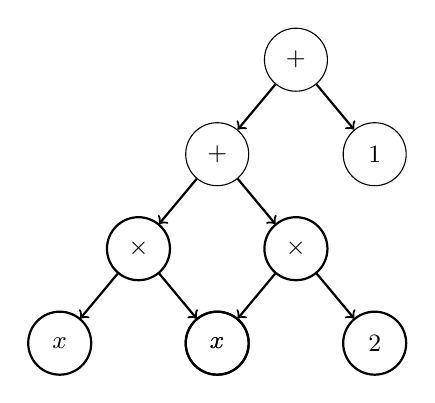
\begin{tikzpicture}[
    level distance=1.2cm,
    sibling distance=2cm,
    every node/.style={draw, circle, minimum size=0.8cm, font=\small},
    edge from parent/.style={draw, ->, thick}
]
    \node {$+$}
        child { node {$+$}
            child { node {$\times$}
                child { node {$x$} }
                child { node {$x$} }
            }
            child { node {$\times$}
                child { node {$x$} }
                child { node {$2$} }
            }
        }
        child { node {$1$} };
\end{tikzpicture}
\end{center}

这棵树的结构就是 $(((x \times x) + (x \times 2)) + 1)$。\textbf{``先乘后加''是在这一步决定的}。

\paragraph{第二步：编译（Compilation）—— 把树变成指令序列}

Python 编译器把 AST 翻译成一串\textbf{字节码指令}（bytecode）。每条指令只做一件很小的事：

\begin{center}
\renewcommand{\arraystretch}{1.3}
\begin{tabular}{cl}
\toprule
\textbf{指令} & \textbf{含义} \\
\midrule
\texttt{LOAD\_FAST x} & 把变量 $x$ 压入栈顶 \\
\texttt{BINARY\_MULTIPLY} & 弹出栈顶两个数，相乘，结果压回栈顶 \\
\texttt{BINARY\_ADD} & 弹出栈顶两个数，相加，结果压回栈顶 \\
\texttt{LOAD\_CONST 2} & 把常数 2 压入栈顶 \\
\bottomrule
\end{tabular}
\end{center}

\paragraph{第三步：执行（Execution）—— 用栈依次运行指令}

解释器维护一个\textbf{栈}（像一摞盘子），严格按字节码顺序执行：

\begin{center}
\small
\renewcommand{\arraystretch}{1.4}
\begin{tabular}{c|l|l}
\toprule
\textbf{步骤} & \textbf{执行的指令} & \textbf{栈的状态}（右边是栈顶） \\
\midrule
1 & \texttt{LOAD\_FAST x} & $[3.0]$ \\
2 & \texttt{LOAD\_FAST x} & $[3.0, 3.0]$ \\
3 & \texttt{BINARY\_MULTIPLY} $\to$ 调用 \texttt{x.\_\_mul\_\_(x)} & $[m_1]$ \quad ($m_1$.data=9.0) \\
\midrule
4 & \texttt{LOAD\_FAST x} & $[m_1, 3.0]$ \\
5 & \texttt{LOAD\_CONST 2} & $[m_1, 3.0, 2]$ \\
6 & \texttt{BINARY\_MULTIPLY} $\to$ 调用 \texttt{x.\_\_mul\_\_(2)} & $[m_1, m_2]$ \quad ($m_2$.data=6.0) \\
\midrule
7 & \texttt{BINARY\_ADD} $\to$ 调用 \texttt{m1.\_\_add\_\_(m2)} & $[s_1]$ \quad ($s_1$.data=15.0) \\
\midrule
8 & \texttt{LOAD\_CONST 1} & $[s_1, 1]$ \\
9 & \texttt{BINARY\_ADD} $\to$ 调用 \texttt{s1.\_\_add\_\_(1)} & $[y]$ \quad ($y$.data=16.0) \\
\bottomrule
\end{tabular}
\end{center}

\textbf{关键洞察}：每次执行 \texttt{BINARY\_MULTIPLY} 或 \texttt{BINARY\_ADD} 时，Python 会调用我们重载的 \texttt{\_\_mul\_\_} 或 \texttt{\_\_add\_\_} 方法。在这些方法里，我们不仅计算了数值，还\textbf{顺便}创建了计算图节点！

\subsection*{真的可以看到字节码吗？}

可以！Python 提供了 \texttt{dis} 模块来查看字节码：

\begin{lstlisting}[style=teaching, language=Python]
import dis

def f(x):
    return x * x + x * 2 + 1

dis.dis(f)
\end{lstlisting}

输出（简化后）：

\begin{lstlisting}[style=teaching, language=Python, numbers=none]
  3           0 LOAD_FAST                0 (x)
              2 LOAD_FAST                0 (x)
              4 BINARY_MULTIPLY              # x * x -> m1

              6 LOAD_FAST                0 (x)
              8 LOAD_CONST               1 (2)
             10 BINARY_MULTIPLY              # x * 2 -> m2

             12 BINARY_ADD                   # m1 + m2 -> s1

             14 LOAD_CONST               2 (1)
             16 BINARY_ADD                   # s1 + 1 -> y

             18 RETURN_VALUE
\end{lstlisting}

这正是第 8 章里逐步搭出计算图的 Step 1--4 图的``官方版本''。

\subsection*{小结}

\begin{center}
\resizebox{\textwidth}{!}{%
\begin{tikzpicture}[
    box/.style={draw, rounded corners, minimum width=3cm, minimum height=1cm, font=\small, align=center},
    arrow/.style={->, thick, >=stealth}
]
    \node[box, fill=blue!10] (src) at (0, 0) {源代码\\{\ttfamily x*x + x*2 + 1}};
    \node[box, fill=green!10] (ast) at (4.5, 0) {抽象语法树\\（确定优先级）};
    \node[box, fill=yellow!10] (bc) at (9, 0) {字节码序列\\（线性指令）};
    \node[box, fill=red!10] (exec) at (13.5, 0) {栈式执行\\（调用重载方法）};
    
    \draw[arrow] (src) -- node[above, font=\scriptsize] {解析} (ast);
    \draw[arrow] (ast) -- node[above, font=\scriptsize] {编译} (bc);
    \draw[arrow] (bc) -- node[above, font=\scriptsize] {执行} (exec);
\end{tikzpicture}}
\end{center}

回顾这三步：\textbf{``先乘后加''}是在\textbf{解析阶段}决定的（构建 AST），\textbf{``从左到右''}是在\textbf{执行阶段}实现的（按字节码顺序）。\textbf{我们没有写任何解析器}，Python 帮我们做完了所有这些工作；我们只需要\textbf{重载运算符}，就能在执行阶段``搭便车''构建计算图。这就是自动微分框架的设计哲学：\textbf{利用宿主语言的表达式求值机制，免费获得计算图构建能力}。PyTorch、JAX、TensorFlow Eager 都是这个思路。


\section*{用 SB3 训练经典控制任务}
\addcontentsline{toc}{section}{用 SB3 训练经典控制任务}
% ------------------------------------------------------------------------------------

第 9 章推导了 DQN、PPO 和 SAC 的更新公式，但真要在一个环境上把它们跑起来，还有经验池、目标网络、裁剪范围这些工程细节要处理。Stable Baselines3（SB3）把这些都封装好了，你只需要选算法、给环境、设超参数。下面的代码展示如何用 SB3 在经典控制任务上训练和对比这三种算法：

\begin{lstlisting}[language=Python, caption={用 SB3 对比三种算法}]
import gymnasium as gym
from stable_baselines3 import DQN, PPO, SAC
import matplotlib.pyplot as plt

# CartPole: 离散动作，适合 DQN 和 PPO
env_discrete = gym.make("CartPole-v1")

# Pendulum: 连续动作，适合 PPO 和 SAC
env_continuous = gym.make("Pendulum-v1")

# --- 训练 DQN（离散动作）---
dqn_model = DQN(
    "MlpPolicy", 
    env_discrete,
    learning_rate=1e-3,
    buffer_size=50000,      # 经验池大小
    learning_starts=1000,   # 开始训练前先收集多少数据
    target_update_interval=500,  # 目标网络更新频率
    verbose=1
)
dqn_model.learn(total_timesteps=20000)

# --- 训练 PPO（通用）---
ppo_model = PPO(
    "MlpPolicy",
    env_discrete,
    learning_rate=3e-4,
    n_steps=2048,           # 每次收集多少步
    batch_size=64,          # 小批量大小
    n_epochs=10,            # 每批数据训练几轮
    clip_range=0.2,         # PPO clip 参数
    verbose=1
)
ppo_model.learn(total_timesteps=20000)

# --- 训练 SAC（连续动作）---
sac_model = SAC(
    "MlpPolicy",
    env_continuous,
    learning_rate=3e-4,
    buffer_size=100000,
    learning_starts=1000,
    tau=0.005,              # 软更新系数
    verbose=1
)
sac_model.learn(total_timesteps=20000)
\end{lstlisting}

\begin{remark}
SB3 的强大之处在于：\textbf{把这里的 \texttt{CartPole} 换成你的自定义环境，代码几乎不用改}。只要你的问题能封装成 Gymnasium 接口——\texttt{reset()} 返回初始状态，\texttt{step(action)} 返回（下一状态，奖励，是否结束，信息）——SB3 就能直接训练。把 CartPole 的物理方程换成飞行器动力学，就是飞行控制；换成流体方程，就是流体控制。
\end{remark}




